% Options for packages loaded elsewhere
\PassOptionsToPackage{unicode}{hyperref}
\PassOptionsToPackage{hyphens}{url}
%
\documentclass[
]{article}
\usepackage{amsmath,amssymb}
\usepackage{iftex}
\ifPDFTeX
  \usepackage[T1]{fontenc}
  \usepackage[utf8]{inputenc}
  \usepackage{textcomp} % provide euro and other symbols
\else % if luatex or xetex
  \usepackage{unicode-math} % this also loads fontspec
  \defaultfontfeatures{Scale=MatchLowercase}
  \defaultfontfeatures[\rmfamily]{Ligatures=TeX,Scale=1}
\fi
\usepackage{lmodern}
\ifPDFTeX\else
  % xetex/luatex font selection
\fi
% Use upquote if available, for straight quotes in verbatim environments
\IfFileExists{upquote.sty}{\usepackage{upquote}}{}
\IfFileExists{microtype.sty}{% use microtype if available
  \usepackage[]{microtype}
  \UseMicrotypeSet[protrusion]{basicmath} % disable protrusion for tt fonts
}{}
\makeatletter
\@ifundefined{KOMAClassName}{% if non-KOMA class
  \IfFileExists{parskip.sty}{%
    \usepackage{parskip}
  }{% else
    \setlength{\parindent}{0pt}
    \setlength{\parskip}{6pt plus 2pt minus 1pt}}
}{% if KOMA class
  \KOMAoptions{parskip=half}}
\makeatother
\usepackage{xcolor}
\usepackage[margin=1in]{geometry}
\usepackage{color}
\usepackage{fancyvrb}
\newcommand{\VerbBar}{|}
\newcommand{\VERB}{\Verb[commandchars=\\\{\}]}
\DefineVerbatimEnvironment{Highlighting}{Verbatim}{commandchars=\\\{\}}
% Add ',fontsize=\small' for more characters per line
\usepackage{framed}
\definecolor{shadecolor}{RGB}{248,248,248}
\newenvironment{Shaded}{\begin{snugshade}}{\end{snugshade}}
\newcommand{\AlertTok}[1]{\textcolor[rgb]{0.94,0.16,0.16}{#1}}
\newcommand{\AnnotationTok}[1]{\textcolor[rgb]{0.56,0.35,0.01}{\textbf{\textit{#1}}}}
\newcommand{\AttributeTok}[1]{\textcolor[rgb]{0.13,0.29,0.53}{#1}}
\newcommand{\BaseNTok}[1]{\textcolor[rgb]{0.00,0.00,0.81}{#1}}
\newcommand{\BuiltInTok}[1]{#1}
\newcommand{\CharTok}[1]{\textcolor[rgb]{0.31,0.60,0.02}{#1}}
\newcommand{\CommentTok}[1]{\textcolor[rgb]{0.56,0.35,0.01}{\textit{#1}}}
\newcommand{\CommentVarTok}[1]{\textcolor[rgb]{0.56,0.35,0.01}{\textbf{\textit{#1}}}}
\newcommand{\ConstantTok}[1]{\textcolor[rgb]{0.56,0.35,0.01}{#1}}
\newcommand{\ControlFlowTok}[1]{\textcolor[rgb]{0.13,0.29,0.53}{\textbf{#1}}}
\newcommand{\DataTypeTok}[1]{\textcolor[rgb]{0.13,0.29,0.53}{#1}}
\newcommand{\DecValTok}[1]{\textcolor[rgb]{0.00,0.00,0.81}{#1}}
\newcommand{\DocumentationTok}[1]{\textcolor[rgb]{0.56,0.35,0.01}{\textbf{\textit{#1}}}}
\newcommand{\ErrorTok}[1]{\textcolor[rgb]{0.64,0.00,0.00}{\textbf{#1}}}
\newcommand{\ExtensionTok}[1]{#1}
\newcommand{\FloatTok}[1]{\textcolor[rgb]{0.00,0.00,0.81}{#1}}
\newcommand{\FunctionTok}[1]{\textcolor[rgb]{0.13,0.29,0.53}{\textbf{#1}}}
\newcommand{\ImportTok}[1]{#1}
\newcommand{\InformationTok}[1]{\textcolor[rgb]{0.56,0.35,0.01}{\textbf{\textit{#1}}}}
\newcommand{\KeywordTok}[1]{\textcolor[rgb]{0.13,0.29,0.53}{\textbf{#1}}}
\newcommand{\NormalTok}[1]{#1}
\newcommand{\OperatorTok}[1]{\textcolor[rgb]{0.81,0.36,0.00}{\textbf{#1}}}
\newcommand{\OtherTok}[1]{\textcolor[rgb]{0.56,0.35,0.01}{#1}}
\newcommand{\PreprocessorTok}[1]{\textcolor[rgb]{0.56,0.35,0.01}{\textit{#1}}}
\newcommand{\RegionMarkerTok}[1]{#1}
\newcommand{\SpecialCharTok}[1]{\textcolor[rgb]{0.81,0.36,0.00}{\textbf{#1}}}
\newcommand{\SpecialStringTok}[1]{\textcolor[rgb]{0.31,0.60,0.02}{#1}}
\newcommand{\StringTok}[1]{\textcolor[rgb]{0.31,0.60,0.02}{#1}}
\newcommand{\VariableTok}[1]{\textcolor[rgb]{0.00,0.00,0.00}{#1}}
\newcommand{\VerbatimStringTok}[1]{\textcolor[rgb]{0.31,0.60,0.02}{#1}}
\newcommand{\WarningTok}[1]{\textcolor[rgb]{0.56,0.35,0.01}{\textbf{\textit{#1}}}}
\usepackage{graphicx}
\makeatletter
\def\maxwidth{\ifdim\Gin@nat@width>\linewidth\linewidth\else\Gin@nat@width\fi}
\def\maxheight{\ifdim\Gin@nat@height>\textheight\textheight\else\Gin@nat@height\fi}
\makeatother
% Scale images if necessary, so that they will not overflow the page
% margins by default, and it is still possible to overwrite the defaults
% using explicit options in \includegraphics[width, height, ...]{}
\setkeys{Gin}{width=\maxwidth,height=\maxheight,keepaspectratio}
% Set default figure placement to htbp
\makeatletter
\def\fps@figure{htbp}
\makeatother
\setlength{\emergencystretch}{3em} % prevent overfull lines
\providecommand{\tightlist}{%
  \setlength{\itemsep}{0pt}\setlength{\parskip}{0pt}}
\setcounter{secnumdepth}{-\maxdimen} % remove section numbering
\ifLuaTeX
  \usepackage{selnolig}  % disable illegal ligatures
\fi
\usepackage{bookmark}
\IfFileExists{xurl.sty}{\usepackage{xurl}}{} % add URL line breaks if available
\urlstyle{same}
\hypersetup{
  pdftitle={Hot stove effect simulations},
  hidelinks,
  pdfcreator={LaTeX via pandoc}}

\title{Hot stove effect simulations}
\author{}
\date{\vspace{-2.5em}}

\begin{document}
\maketitle

\subsection{Load libraries}\label{load-libraries}

The libraries needed in this project are mainly dplyr for data wrangling
and ggplot2 for data visualization. Both are part of the collection of
packages known as the tidyverse, which we will load next.

\begin{Shaded}
\begin{Highlighting}[]
\FunctionTok{library}\NormalTok{(tidyverse)}
\end{Highlighting}
\end{Shaded}

\subsection{Define simulation
parameters}\label{define-simulation-parameters}

\begin{Shaded}
\begin{Highlighting}[]
\DocumentationTok{\#\#\#\#DEFINE GRAPHICAL PARAMETERS\#\#\#\#}
\NormalTok{axeswidth }\OtherTok{\textless{}{-}} \FloatTok{0.5}
\NormalTok{genplotwidth }\OtherTok{\textless{}{-}} \DecValTok{1}
\NormalTok{size\_indivline }\OtherTok{\textless{}{-}} \FloatTok{0.2}
\NormalTok{size\_indivdot }\OtherTok{\textless{}{-}} \FloatTok{1.5}
\NormalTok{size\_sumdot }\OtherTok{\textless{}{-}} \DecValTok{4}
\NormalTok{size\_line\_lineplot }\OtherTok{\textless{}{-}} \FloatTok{0.5}
\NormalTok{stroke\_indivdot }\OtherTok{\textless{}{-}} \FloatTok{0.5}
\NormalTok{stroke\_sumdot }\OtherTok{\textless{}{-}} \FloatTok{0.5}
\NormalTok{sizefont }\OtherTok{\textless{}{-}} \DecValTok{12}
\NormalTok{sizeannot }\OtherTok{\textless{}{-}} \DecValTok{4}
\NormalTok{smoothvalue }\OtherTok{\textless{}{-}} \DecValTok{1}\SpecialCharTok{/}\DecValTok{2}

\FunctionTok{theme\_set}\NormalTok{ (}\FunctionTok{theme\_classic}\NormalTok{(}\DecValTok{14}\NormalTok{) }\SpecialCharTok{+} \FunctionTok{theme}\NormalTok{(}\AttributeTok{axis.line.x =} \FunctionTok{element\_line}\NormalTok{(}\AttributeTok{colour =} \StringTok{\textquotesingle{}black\textquotesingle{}}\NormalTok{, }\AttributeTok{linewidth=}\NormalTok{axeswidth, }\AttributeTok{linetype=}\StringTok{\textquotesingle{}solid\textquotesingle{}}\NormalTok{),}
                                     \AttributeTok{axis.line.y =} \FunctionTok{element\_line}\NormalTok{(}\AttributeTok{colour =} \StringTok{\textquotesingle{}black\textquotesingle{}}\NormalTok{, }\AttributeTok{linewidth=}\NormalTok{axeswidth, }\AttributeTok{linetype=}\StringTok{\textquotesingle{}solid\textquotesingle{}}\NormalTok{),}
                                     \AttributeTok{axis.ticks =} \FunctionTok{element\_line}\NormalTok{(}\AttributeTok{color=}\StringTok{"black"}\NormalTok{, }\AttributeTok{linewidth=}\NormalTok{axeswidth),}
                                     \AttributeTok{axis.text.x =} \FunctionTok{element\_text}\NormalTok{(}\AttributeTok{color=}\StringTok{"black"}\NormalTok{),}
                                     \AttributeTok{axis.text.y =} \FunctionTok{element\_text}\NormalTok{(}\AttributeTok{color=}\StringTok{"black"}\NormalTok{),}
                                     \AttributeTok{text =} \FunctionTok{element\_text}\NormalTok{(}\AttributeTok{family =} \StringTok{"Helvetica"}\NormalTok{)))}

\NormalTok{hue\_arm1 }\OtherTok{\textless{}{-}}\StringTok{"\#bf812d"}
\NormalTok{hue\_arm2 }\OtherTok{\textless{}{-}} \StringTok{"\#01665e"}
\NormalTok{paltau\_color }\OtherTok{\textless{}{-}} \FunctionTok{scale\_color\_manual}\NormalTok{(}\AttributeTok{name =} \FunctionTok{expression}\NormalTok{(}\StringTok{"\textbackslash{}u03C4"}\NormalTok{),}\AttributeTok{values =}  \FunctionTok{c}\NormalTok{(}\StringTok{"\#df65b0"}\NormalTok{,}\StringTok{"\#e7298a"}\NormalTok{,}\StringTok{"\#ce1256"}\NormalTok{,}\StringTok{"\#980043"}\NormalTok{) )}
\NormalTok{paltau\_fill }\OtherTok{\textless{}{-}} \FunctionTok{scale\_fill\_manual}\NormalTok{(}\AttributeTok{name =} \FunctionTok{expression}\NormalTok{(}\StringTok{"\textbackslash{}u03C4"}\NormalTok{),}\AttributeTok{values =}  \FunctionTok{c}\NormalTok{(}\StringTok{"\#df65b0"}\NormalTok{,}\StringTok{"\#e7298a"}\NormalTok{,}\StringTok{"\#ce1256"}\NormalTok{,}\StringTok{"\#980043"}\NormalTok{) )}

\NormalTok{scalex\_trials }\OtherTok{\textless{}{-}}  \FunctionTok{scale\_x\_continuous}\NormalTok{(}\AttributeTok{breaks =} \FunctionTok{c}\NormalTok{(}\DecValTok{5}\NormalTok{, }\DecValTok{10}\NormalTok{, }\DecValTok{15}\NormalTok{, }\DecValTok{20}\NormalTok{, }\DecValTok{25}\NormalTok{), }\AttributeTok{labels =} \FunctionTok{c}\NormalTok{(}\DecValTok{5}\NormalTok{, }\DecValTok{10}\NormalTok{, }\DecValTok{15}\NormalTok{, }\DecValTok{20}\NormalTok{, }\DecValTok{25}\NormalTok{))}
\end{Highlighting}
\end{Shaded}

\subsection{Define simulation
parameters}\label{define-simulation-parameters-1}

\begin{Shaded}
\begin{Highlighting}[]
\DocumentationTok{\#\#\#\#DEFINE SIMULATION PARAMETERS\#\#\#\#}
\NormalTok{nsims }\OtherTok{\textless{}{-}} \DecValTok{1000} \CommentTok{\#number of simulations per tau value}
\NormalTok{ntrialsperblock }\OtherTok{\textless{}{-}} \DecValTok{25} \CommentTok{\#number of trials per simulation (aka horizon)}
\NormalTok{euler }\OtherTok{\textless{}{-}} \FunctionTok{exp}\NormalTok{(}\DecValTok{1}\NormalTok{) }\CommentTok{\#e, so we can use it later}

\NormalTok{mu\_arm1 }\OtherTok{\textless{}{-}} \DecValTok{5}
\NormalTok{mu\_arm2 }\OtherTok{\textless{}{-}} \SpecialCharTok{{-}}\DecValTok{5}
\NormalTok{sigma\_arms }\OtherTok{\textless{}{-}} \DecValTok{15}
\NormalTok{rewcap\_up\_arm1 }\OtherTok{\textless{}{-}}\NormalTok{ mu\_arm1 }\SpecialCharTok{+}\NormalTok{ (sigma\_arms}\SpecialCharTok{*}\DecValTok{3}\NormalTok{) }\CommentTok{\#for arm 1, truncating reward so it cannot be bigger than mean plus minus 3 SDs}
\NormalTok{rewcap\_low\_arm1 }\OtherTok{\textless{}{-}}\NormalTok{ mu\_arm1 }\SpecialCharTok{{-}}\NormalTok{ (sigma\_arms}\SpecialCharTok{*}\DecValTok{3}\NormalTok{) }\CommentTok{\#for arm 1, truncating reward so it cannot be smaller than mean plus minus 3 SDs}
\NormalTok{rewcap\_up\_arm2 }\OtherTok{\textless{}{-}}\NormalTok{ mu\_arm2 }\SpecialCharTok{+}\NormalTok{ (sigma\_arms}\SpecialCharTok{*}\DecValTok{3}\NormalTok{) }\CommentTok{\#same as above, for arm 2}
\NormalTok{rewcap\_low\_arm2 }\OtherTok{\textless{}{-}}\NormalTok{ mu\_arm2 }\SpecialCharTok{{-}}\NormalTok{ (sigma\_arms}\SpecialCharTok{*}\DecValTok{3}\NormalTok{) }\CommentTok{\#same as above, for arm 2}

\NormalTok{vectau }\OtherTok{\textless{}{-}} \FunctionTok{c}\NormalTok{(}\DecValTok{2}\NormalTok{,}\DecValTok{10}\NormalTok{,}\DecValTok{18}\NormalTok{,}\DecValTok{26}\NormalTok{) }\CommentTok{\#vector of taus with which we will run simulations \#10}
\end{Highlighting}
\end{Shaded}

\begin{Shaded}
\begin{Highlighting}[]
\NormalTok{figure\_gaussians }\OtherTok{\textless{}{-}} \FunctionTok{ggplot}\NormalTok{() }\SpecialCharTok{+}
  \FunctionTok{geom\_function}\NormalTok{(}
    \AttributeTok{data =} \FunctionTok{data.frame}\NormalTok{(}\AttributeTok{x =} \FunctionTok{c}\NormalTok{(rewcap\_low\_arm1, rewcap\_up\_arm1)), }\FunctionTok{aes}\NormalTok{(}\AttributeTok{x =}\NormalTok{ x), }\AttributeTok{fun =}\NormalTok{ dnorm,}
    \AttributeTok{args =} \FunctionTok{list}\NormalTok{(}\AttributeTok{mean =}\NormalTok{ mu\_arm1, }\AttributeTok{sd =}\NormalTok{ sigma\_arms), }\AttributeTok{size =} \DecValTok{1}\NormalTok{, }\AttributeTok{color =}\NormalTok{ hue\_arm1) }\SpecialCharTok{+}
  \FunctionTok{geom\_function}\NormalTok{(}
    \AttributeTok{data =} \FunctionTok{data.frame}\NormalTok{(}\AttributeTok{x =} \FunctionTok{c}\NormalTok{(rewcap\_low\_arm2, rewcap\_up\_arm2)), }\FunctionTok{aes}\NormalTok{(}\AttributeTok{x =}\NormalTok{ x), }\AttributeTok{fun =}\NormalTok{ dnorm,}
    \AttributeTok{args =} \FunctionTok{list}\NormalTok{(}\AttributeTok{mean =}\NormalTok{ mu\_arm2, }\AttributeTok{sd =}\NormalTok{ sigma\_arms), }\AttributeTok{size =} \DecValTok{1}\NormalTok{, }\AttributeTok{color =}\NormalTok{ hue\_arm2) }\SpecialCharTok{+}
  \FunctionTok{geom\_vline}\NormalTok{(}\AttributeTok{xintercept =}\NormalTok{ mu\_arm1, }\AttributeTok{color =}\NormalTok{ hue\_arm1, }\AttributeTok{size =} \DecValTok{1}\NormalTok{, }\AttributeTok{linetype =} \StringTok{"dashed"}\NormalTok{) }\SpecialCharTok{+} 
  \FunctionTok{geom\_vline}\NormalTok{(}\AttributeTok{xintercept =}\NormalTok{ mu\_arm2, }\AttributeTok{color =}\NormalTok{ hue\_arm2, }\AttributeTok{size =} \DecValTok{1}\NormalTok{, }\AttributeTok{linetype =} \StringTok{"dashed"}\NormalTok{) }\SpecialCharTok{+}
  \FunctionTok{xlab}\NormalTok{(}\StringTok{"Reward"}\NormalTok{) }\SpecialCharTok{+} 
  \FunctionTok{ylab}\NormalTok{(}\StringTok{"Probability"}\NormalTok{) }\SpecialCharTok{+}
  \FunctionTok{ylim}\NormalTok{(}\DecValTok{0}\NormalTok{, }\ConstantTok{NA}\NormalTok{)}
\end{Highlighting}
\end{Shaded}

\begin{verbatim}
## Warning: Using `size` aesthetic for lines was deprecated in ggplot2 3.4.0.
## i Please use `linewidth` instead.
## This warning is displayed once every 8 hours.
## Call `lifecycle::last_lifecycle_warnings()` to see where this warning was
## generated.
\end{verbatim}

\begin{Shaded}
\begin{Highlighting}[]
\NormalTok{figure\_gaussians}
\end{Highlighting}
\end{Shaded}

\includegraphics{hot_stove_sims_files/figure-latex/unnamed-chunk-4-1.pdf}

\subsection{Define functions}\label{define-functions}

\begin{Shaded}
\begin{Highlighting}[]
\CommentTok{\#function: generate rounded random normal samples with a given mean, sd and minimum and maximum bounds}
\NormalTok{normsamp\_round\_bounded }\OtherTok{\textless{}{-}} \ControlFlowTok{function}\NormalTok{(}
\NormalTok{    mean, }\CommentTok{\#mean}
\NormalTok{    stddev, }\CommentTok{\#standard deviation}
\NormalTok{    nsamples, }\CommentTok{\#number of samples to generate}
\NormalTok{    minval, }\CommentTok{\#minimum value a sample can take}
\NormalTok{    maxval) \{ }\CommentTok{\#maximum value a sample can take}
  
\NormalTok{  finarr }\OtherTok{\textless{}{-}} \ConstantTok{NULL} \CommentTok{\#predefining final array so we can append to it}
  
  \ControlFlowTok{for}\NormalTok{ (g }\ControlFlowTok{in} \DecValTok{1}\SpecialCharTok{:}\NormalTok{nsamples)\{}
    
    \ControlFlowTok{repeat}\NormalTok{\{ }\CommentTok{\#repeat generating sample as long as it is not within min and max bounds}
\NormalTok{      cursample }\OtherTok{\textless{}{-}} \FunctionTok{rnorm}\NormalTok{(}\AttributeTok{n =} \DecValTok{1}\NormalTok{, }\AttributeTok{mean =}\NormalTok{ mean, }\AttributeTok{sd =}\NormalTok{ stddev) }\CommentTok{\#generate sample}
      
      \ControlFlowTok{if}\NormalTok{(cursample }\SpecialCharTok{\textgreater{}=}\NormalTok{ minval }\SpecialCharTok{\&}\NormalTok{ cursample }\SpecialCharTok{\textless{}=}\NormalTok{ maxval)\{ }\CommentTok{\#if within bounds, no need to resample}
        \ControlFlowTok{break}
\NormalTok{      \}\}}
    
\NormalTok{    cursample\_rounded }\OtherTok{\textless{}{-}} \FunctionTok{round}\NormalTok{(cursample) }\CommentTok{\#round current sample}
\NormalTok{    finarr }\OtherTok{\textless{}{-}} \FunctionTok{c}\NormalTok{(finarr,cursample\_rounded) }\CommentTok{\#append current sample to final array}
\NormalTok{  \}}
  \FunctionTok{return}\NormalTok{(finarr)}
\NormalTok{\} }\CommentTok{\#end of function normsamp\_round\_bounded}
\end{Highlighting}
\end{Shaded}

Second function

\begin{Shaded}
\begin{Highlighting}[]
\CommentTok{\#function: simulate two{-}armed bandit games where agent chooses based on softmax and outcomes are those generated by using normsamp\_round\_bounded function}
\NormalTok{do\_softmax\_twoarms }\OtherTok{\textless{}{-}} \ControlFlowTok{function}\NormalTok{(}
\NormalTok{    nsims, }\CommentTok{\#number of simulations to run within each tau value}
\NormalTok{    vectau, }\CommentTok{\#vector with values of tau to run simulations with}
\NormalTok{    ntrialsperblock, }\CommentTok{\#number of trials (choices) per block}
\NormalTok{    mu\_arm1, }\CommentTok{\#mean for arm 1}
\NormalTok{    mu\_arm2, }\CommentTok{\#mean for arm 2}
\NormalTok{    sigma\_arms, }\CommentTok{\#standard deviation shared by both arms}
\NormalTok{    rewcap\_low\_arm1, }\CommentTok{\#minimum value reward (outcome) for arm 1 can take}
\NormalTok{    rewcap\_up\_arm1, }\CommentTok{\#maximum value reward (outcome) for arm 1 can take}
\NormalTok{    rewcap\_low\_arm2, }\CommentTok{\#same, for arm 2}
\NormalTok{    rewcap\_up\_arm2) \{}
  
\NormalTok{  finaldf }\OtherTok{\textless{}{-}} \ConstantTok{NULL} \CommentTok{\#predefine final data frame so we can append to it}
  
  \ControlFlowTok{for}\NormalTok{ (g }\ControlFlowTok{in} \DecValTok{1}\SpecialCharTok{:}\FunctionTok{length}\NormalTok{(vectau))\{}
\NormalTok{    curtau }\OtherTok{\textless{}{-}}\NormalTok{ vectau[g] }\CommentTok{\#current tau value}
    \ControlFlowTok{for}\NormalTok{ (h }\ControlFlowTok{in} \DecValTok{1}\SpecialCharTok{:}\NormalTok{nsims)\{ }
      
\NormalTok{      condmet }\OtherTok{\textless{}{-}} \DecValTok{0} \CommentTok{\#predefining condition met to 0}
      \ControlFlowTok{while}\NormalTok{ (condmet }\SpecialCharTok{\textless{}} \DecValTok{1}\NormalTok{) \{ }\CommentTok{\#through while loop, we force mean reward for any simulation to be higher for arm A than for arm B, otherwise we generate reward samples again}
\NormalTok{        currew\_arm1 }\OtherTok{\textless{}{-}} \FunctionTok{normsamp\_round\_bounded}\NormalTok{(}
          \AttributeTok{mean =}\NormalTok{ mu\_arm1,}
          \AttributeTok{stddev =}\NormalTok{ sigma\_arms, }
          \AttributeTok{nsamples =}\NormalTok{ ntrialsperblock, }
          \AttributeTok{minval =}\NormalTok{ rewcap\_low\_arm1, }
          \AttributeTok{maxval =}\NormalTok{ rewcap\_up\_arm1)}\CommentTok{\#generating reward for arm 1, if selected. Samples are within bounds (otherwise resampled) and rounded to nearest integer}
        
\NormalTok{        currew\_arm2 }\OtherTok{\textless{}{-}} \FunctionTok{normsamp\_round\_bounded}\NormalTok{(}
          \AttributeTok{mean =}\NormalTok{ mu\_arm2,}
          \AttributeTok{stddev =}\NormalTok{ sigma\_arms, }
          \AttributeTok{nsamples =}\NormalTok{ ntrialsperblock, }
          \AttributeTok{minval =}\NormalTok{ rewcap\_low\_arm2, }
          \AttributeTok{maxval =}\NormalTok{ rewcap\_up\_arm2)}\CommentTok{\#same, for arm 2}
        
        \ControlFlowTok{if}\NormalTok{ (}\FunctionTok{mean}\NormalTok{(currew\_arm1) }\SpecialCharTok{\textgreater{}} \FunctionTok{mean}\NormalTok{(currew\_arm2)) \{ }\CommentTok{\#if mean reward for arm 1 is higer}
\NormalTok{          condmet }\OtherTok{\textless{}{-}} \DecValTok{1} \CommentTok{\#condition is met, so break the while loop}
\NormalTok{        \}}
\NormalTok{      \} }\CommentTok{\#end of while loop}
      
\NormalTok{      curdf }\OtherTok{\textless{}{-}} \FunctionTok{tibble}\NormalTok{( }\CommentTok{\#dataframe for current simulation, some variables we already know, some we preallocate to replace later}
        \AttributeTok{trial =} \DecValTok{1}\SpecialCharTok{:}\NormalTok{ntrialsperblock, }\CommentTok{\#trial number}
        \AttributeTok{tau =}\NormalTok{ curtau, }\CommentTok{\#tau value}
        \AttributeTok{sim=}\NormalTok{h, }\CommentTok{\#simulation number}
        \AttributeTok{rew\_arm1 =}\NormalTok{ currew\_arm1, }\CommentTok{\#reward for that trial if picking arm 1}
        \AttributeTok{rew\_arm2 =}\NormalTok{ currew\_arm2, }\CommentTok{\#same for arm 2}
        \AttributeTok{estmu\_arm1 =} \ConstantTok{NA}\NormalTok{, }\CommentTok{\#estimated value for arm 1}
        \AttributeTok{estmu\_arm2 =} \ConstantTok{NA}\NormalTok{, }\CommentTok{\#same for arm 2}
        \AttributeTok{exploit\_choice =} \ConstantTok{NA}\NormalTok{, }\CommentTok{\#exploration or exploitation}
        \AttributeTok{choice =} \ConstantTok{NA}\NormalTok{, }\CommentTok{\#arm choice}
        \AttributeTok{rew\_obs =} \ConstantTok{NA}\NormalTok{) }\CommentTok{\#observed reward}
      
      \ControlFlowTok{for}\NormalTok{ (i }\ControlFlowTok{in} \DecValTok{1}\SpecialCharTok{:}\NormalTok{ntrialsperblock)\{ }
        
        \ControlFlowTok{if}\NormalTok{ (i }\SpecialCharTok{\textgreater{}} \DecValTok{1}\NormalTok{)\{ }\CommentTok{\#if there was already a choice for an arm, we can calculate estimated value for that arm}
          
\NormalTok{          estmu\_arm1 }\OtherTok{\textless{}{-}}\NormalTok{ curdf }\SpecialCharTok{\%\textgreater{}\%} 
            \FunctionTok{filter}\NormalTok{(choice}\SpecialCharTok{==}\DecValTok{1} \SpecialCharTok{\&}\NormalTok{ trial }\SpecialCharTok{\textless{}}\NormalTok{ i) }\SpecialCharTok{\%\textgreater{}\%} \CommentTok{\#choose all trials so far where choice was arm 1}
            \FunctionTok{summarise}\NormalTok{(}\AttributeTok{parobarm =} \FunctionTok{mean}\NormalTok{(rew\_arm1, }\AttributeTok{na.rm =} \ConstantTok{TRUE}\NormalTok{)) }\CommentTok{\#average reward for those trials}
\NormalTok{          estmu\_arm1 }\OtherTok{\textless{}{-}}\NormalTok{ estmu\_arm1}\SpecialCharTok{$}\NormalTok{parobarm }\CommentTok{\#the average calculated above is the estimated value for arm 1}
          
\NormalTok{          estmu\_arm2 }\OtherTok{\textless{}{-}}\NormalTok{ curdf }\SpecialCharTok{\%\textgreater{}\%} \CommentTok{\#same for arm 2}
            \FunctionTok{filter}\NormalTok{(choice}\SpecialCharTok{==}\DecValTok{2} \SpecialCharTok{\&}\NormalTok{ trial }\SpecialCharTok{\textless{}}\NormalTok{ i) }\SpecialCharTok{\%\textgreater{}\%} 
            \FunctionTok{summarise}\NormalTok{(}\AttributeTok{parobarm =} \FunctionTok{mean}\NormalTok{(rew\_arm2, }\AttributeTok{na.rm =} \ConstantTok{TRUE}\NormalTok{))}
\NormalTok{          estmu\_arm2 }\OtherTok{\textless{}{-}}\NormalTok{ estmu\_arm2}\SpecialCharTok{$}\NormalTok{parobarm}
          
          \ControlFlowTok{if}\NormalTok{ (}\FunctionTok{is.nan}\NormalTok{(estmu\_arm1) }\SpecialCharTok{==} \ConstantTok{FALSE}\NormalTok{)\{ }\CommentTok{\#assign value to df if it is not a NaN}
\NormalTok{            curdf}\SpecialCharTok{$}\NormalTok{estmu\_arm1[i] }\OtherTok{\textless{}{-}}\NormalTok{ estmu\_arm1}
\NormalTok{          \} }
          \ControlFlowTok{if}\NormalTok{ (}\FunctionTok{is.nan}\NormalTok{(estmu\_arm2) }\SpecialCharTok{==} \ConstantTok{FALSE}\NormalTok{)\{ }\CommentTok{\#same for arm 2}
\NormalTok{            curdf}\SpecialCharTok{$}\NormalTok{estmu\_arm2[i] }\OtherTok{\textless{}{-}}\NormalTok{ estmu\_arm2}
\NormalTok{          \} }
\NormalTok{        \} }\CommentTok{\#end of value estimation}
        
        \ControlFlowTok{if}\NormalTok{ (i }\SpecialCharTok{==} \DecValTok{1} \SpecialCharTok{||} \FunctionTok{is.na}\NormalTok{(curdf}\SpecialCharTok{$}\NormalTok{estmu\_arm1[i]) }\SpecialCharTok{||} \FunctionTok{is.na}\NormalTok{(curdf}\SpecialCharTok{$}\NormalTok{estmu\_arm2[i]) }\SpecialCharTok{||}\NormalTok{ curdf}\SpecialCharTok{$}\NormalTok{estmu\_arm1[i] }\SpecialCharTok{==}\NormalTok{ curdf}\SpecialCharTok{$}\NormalTok{estmu\_arm2[i])\{}\CommentTok{\#first trial, or if estimated probs of both options are the same, or if any option has not been chosen yet}
          
          \CommentTok{\#no representation of either arm value, so make choice based on coin flip}
\NormalTok{          choice }\OtherTok{\textless{}{-}} \FunctionTok{sample}\NormalTok{(}\FunctionTok{c}\NormalTok{(}\DecValTok{1}\NormalTok{,}\DecValTok{2}\NormalTok{), }\AttributeTok{size =} \DecValTok{1}\NormalTok{) }\CommentTok{\#flip a coin to choose an option}
\NormalTok{          curdf}\SpecialCharTok{$}\NormalTok{choice[i] }\OtherTok{\textless{}{-}}\NormalTok{ choice }\CommentTok{\#choosing arm 1 = 1, choosing arm 2 = 2}
          
\NormalTok{        \} }\ControlFlowTok{else}\NormalTok{ \{}\CommentTok{\#if it is not first trial and we have representation of value for both arms, base decision on estimated probability for both arms}
          
\NormalTok{          soft\_prob\_arm1 }\OtherTok{\textless{}{-}}\NormalTok{ (euler}\SpecialCharTok{\^{}}\NormalTok{(estmu\_arm1}\SpecialCharTok{/}\NormalTok{curtau))}\SpecialCharTok{/}\NormalTok{((euler}\SpecialCharTok{\^{}}\NormalTok{(estmu\_arm1}\SpecialCharTok{/}\NormalTok{curtau))}\SpecialCharTok{+}\NormalTok{(euler}\SpecialCharTok{\^{}}\NormalTok{(estmu\_arm2}\SpecialCharTok{/}\NormalTok{curtau)))}\CommentTok{\#in softmax, probability of choosing arm 1 depends on estimated probability of each arm and tau (temperature) parameter}
          \CommentTok{\#soft\_prob\_arm1 \textless{}{-} exp(estmu\_arm1*curtau) / (exp(estmu\_arm1*curtau) + exp(estmu\_arm2*curtau)) \#standard way of operationalizing softmax}
          
\NormalTok{          choice }\OtherTok{\textless{}{-}} \FunctionTok{rbinom}\NormalTok{(}\AttributeTok{n =} \DecValTok{1}\NormalTok{, }\AttributeTok{size =} \DecValTok{1}\NormalTok{, }\AttributeTok{prob =}\NormalTok{ (}\DecValTok{1}\SpecialCharTok{{-}}\NormalTok{soft\_prob\_arm1))}\SpecialCharTok{+}\DecValTok{1}\CommentTok{\#choosing arm 1 (1) or 2 (2)?}
\NormalTok{          curdf}\SpecialCharTok{$}\NormalTok{choice[i] }\OtherTok{\textless{}{-}}\NormalTok{ choice}\CommentTok{\#choosing arm 1 = 1, choosing arm 2 = 2}
          
          \ControlFlowTok{if}\NormalTok{ (choice }\SpecialCharTok{==} \DecValTok{1}\NormalTok{)\{}\CommentTok{\#arm 1 chosen}
            \ControlFlowTok{if}\NormalTok{(curdf}\SpecialCharTok{$}\NormalTok{estmu\_arm1[i] }\SpecialCharTok{\textgreater{}}\NormalTok{ curdf}\SpecialCharTok{$}\NormalTok{estmu\_arm2[i])\{}\CommentTok{\#if prob arm 1 higher than arm 2, exploitation took place}
\NormalTok{              curdf}\SpecialCharTok{$}\NormalTok{exploit\_choice[i] }\OtherTok{\textless{}{-}} \DecValTok{1}
\NormalTok{            \}}\ControlFlowTok{else}\NormalTok{\{}\CommentTok{\#exploration took place}
\NormalTok{              curdf}\SpecialCharTok{$}\NormalTok{exploit\_choice[i] }\OtherTok{\textless{}{-}} \DecValTok{0}
\NormalTok{            \}}
            
\NormalTok{          \}}\ControlFlowTok{else}\NormalTok{\{}\CommentTok{\#arm 2 chosen}
            \ControlFlowTok{if}\NormalTok{(curdf}\SpecialCharTok{$}\NormalTok{estmu\_arm1[i] }\SpecialCharTok{\textless{}}\NormalTok{ curdf}\SpecialCharTok{$}\NormalTok{estmu\_arm2[i])\{}\CommentTok{\#if prob arm 2 higher than arm 1, exploitation took place}
\NormalTok{              curdf}\SpecialCharTok{$}\NormalTok{exploit\_choice[i] }\OtherTok{\textless{}{-}} \DecValTok{1}
\NormalTok{            \}}\ControlFlowTok{else}\NormalTok{\{}\CommentTok{\#exploration took place}
\NormalTok{              curdf}\SpecialCharTok{$}\NormalTok{exploit\_choice[i] }\OtherTok{\textless{}{-}} \DecValTok{0}
\NormalTok{            \}}
\NormalTok{          \}}
          
\NormalTok{        \} }\CommentTok{\#end not first trial}
        
        \ControlFlowTok{if}\NormalTok{ (choice }\SpecialCharTok{==} \DecValTok{1}\NormalTok{)\{}\CommentTok{\#arm 1 chosen}
\NormalTok{          curdf}\SpecialCharTok{$}\NormalTok{rew\_obs[i] }\OtherTok{\textless{}{-}}\NormalTok{ curdf}\SpecialCharTok{$}\NormalTok{rew\_arm1[i] }\CommentTok{\#reward is that for arm 1}
\NormalTok{        \}}\ControlFlowTok{else}\NormalTok{ \{}\CommentTok{\#arm 2 chosen}
\NormalTok{          curdf}\SpecialCharTok{$}\NormalTok{rew\_obs[i] }\OtherTok{\textless{}{-}}\NormalTok{ curdf}\SpecialCharTok{$}\NormalTok{rew\_arm2[i] }\CommentTok{\#reward is that for arm 2}
\NormalTok{        \}}
        
\NormalTok{      \}}\CommentTok{\#end that simulation number within current tau value}
\NormalTok{      finaldf }\OtherTok{\textless{}{-}} \FunctionTok{rbind}\NormalTok{(finaldf,curdf) }\CommentTok{\#append current df to final df}
\NormalTok{    \}}\CommentTok{\#end simulations for current tau value}
    
\NormalTok{  \}}\CommentTok{\#end tau loop}
  
  \FunctionTok{return}\NormalTok{(finaldf)}
\NormalTok{\} }\CommentTok{\#end of function do\_softmax\_twoarms}
\end{Highlighting}
\end{Shaded}

\subsection{Simulate}\label{simulate}

\begin{Shaded}
\begin{Highlighting}[]
\CommentTok{\# simsdf \textless{}{-} do\_softmax\_twoarms (nsims = nsims,}
\CommentTok{\#                                     vectau = vectau,}
\CommentTok{\#                                     ntrialsperblock = ntrialsperblock,}
\CommentTok{\#                                     mu\_arm1 = mu\_arm1,}
\CommentTok{\#                                     mu\_arm2 =mu\_arm2,}
\CommentTok{\#                                     sigma\_arms = sigma\_arms,}
\CommentTok{\#                                     rewcap\_low\_arm1 = rewcap\_low\_arm1,}
\CommentTok{\#                                     rewcap\_up\_arm1 = rewcap\_up\_arm1,}
\CommentTok{\#                                     rewcap\_low\_arm2 = rewcap\_low\_arm2,}
\CommentTok{\#                                     rewcap\_up\_arm2 = rewcap\_up\_arm2)}

\CommentTok{\#write.csv(simsdf, file = "simsdf.csv", row.names = FALSE)}
\NormalTok{simsdf }\OtherTok{\textless{}{-}} \FunctionTok{read.csv}\NormalTok{(}\StringTok{"simsdf.csv"}\NormalTok{)}
\end{Highlighting}
\end{Shaded}

\subsection{Summarise}\label{summarise}

\begin{Shaded}
\begin{Highlighting}[]
\NormalTok{simsdf }\OtherTok{\textless{}{-}}\NormalTok{ simsdf }\SpecialCharTok{\%\textgreater{}\%}
  \FunctionTok{group\_by}\NormalTok{(tau,sim) }\SpecialCharTok{\%\textgreater{}\%}
  \FunctionTok{mutate}\NormalTok{(}\AttributeTok{choice\_arm1 =} \FunctionTok{ifelse}\NormalTok{(choice}\SpecialCharTok{==}\DecValTok{1}\NormalTok{,}\DecValTok{1}\NormalTok{,}\DecValTok{0}\NormalTok{)) }\SpecialCharTok{\%\textgreater{}\%} \CommentTok{\#if 1, arm 1 was chosen}
  \FunctionTok{mutate}\NormalTok{(}\AttributeTok{cum\_choice\_arm1 =} \FunctionTok{cumsum}\NormalTok{(choice\_arm1)}\SpecialCharTok{/}\NormalTok{trial, }\CommentTok{\#cumulative of previous}
         \AttributeTok{cumrew=}\FunctionTok{cumsum}\NormalTok{(rew\_obs), }\CommentTok{\#reward so far within that block}
         \AttributeTok{rew\_obs\_arm1=}\FunctionTok{ifelse}\NormalTok{(choice}\SpecialCharTok{==}\DecValTok{1}\NormalTok{,rew\_obs,}\ConstantTok{NA}\NormalTok{), }\CommentTok{\#reward so far after that trial within that block after choosing arm 1}
         \AttributeTok{rew\_obs\_arm2=}\FunctionTok{ifelse}\NormalTok{(choice}\SpecialCharTok{==}\DecValTok{2}\NormalTok{,rew\_obs,}\ConstantTok{NA}\NormalTok{), }\CommentTok{\#same for arm 2}
         \AttributeTok{cumrew\_obs\_arm1=}\FunctionTok{cumsum}\NormalTok{(}\FunctionTok{ifelse}\NormalTok{(}\FunctionTok{is.na}\NormalTok{(rew\_obs\_arm1), }\DecValTok{0}\NormalTok{, rew\_obs\_arm1)),   }\CommentTok{\#cumulative of previous, while ignoring NAs}
                                \AttributeTok{cumrew\_obs\_arm2=}\FunctionTok{cumsum}\NormalTok{(}\FunctionTok{ifelse}\NormalTok{(}\FunctionTok{is.na}\NormalTok{(rew\_obs\_arm2), }\DecValTok{0}\NormalTok{, rew\_obs\_arm2)), }\CommentTok{\#same for arm 2}
         \AttributeTok{difrew\_obs\_arm1min2 =}\NormalTok{ cumrew\_obs\_arm1 }\SpecialCharTok{{-}}\NormalTok{ cumrew\_obs\_arm2, }\CommentTok{\#difference observed reward so far arm 1 minus 2}
         \AttributeTok{difrew\_obs\_arm1min2\_lag =} \FunctionTok{lag}\NormalTok{(difrew\_obs\_arm1min2), }\CommentTok{\#lag of previous}
         \AttributeTok{choice\_bestobsrewarm =} \FunctionTok{ifelse}\NormalTok{(choice}\SpecialCharTok{==}\DecValTok{1} \SpecialCharTok{\&}\NormalTok{ difrew\_obs\_arm1min2\_lag}\SpecialCharTok{\textgreater{}}\DecValTok{0}\NormalTok{,}\DecValTok{1}\NormalTok{,}
                                       \FunctionTok{ifelse}\NormalTok{(choice}\SpecialCharTok{==}\DecValTok{2} \SpecialCharTok{\&}\NormalTok{ difrew\_obs\_arm1min2\_lag}\SpecialCharTok{\textless{}}\DecValTok{0}\NormalTok{,}\DecValTok{1}\NormalTok{,}\DecValTok{0}\NormalTok{))) }\CommentTok{\#if arm with highest reward so far has been picked, 1, otherwise 0 (including any choice when reward the same so far for both options, like in trial 1) }
\NormalTok{  sims\_sum\_df }\OtherTok{\textless{}{-}}\NormalTok{ simsdf }\SpecialCharTok{\%\textgreater{}\%}
  \FunctionTok{group\_by}\NormalTok{(tau,trial) }\SpecialCharTok{\%\textgreater{}\%} 
  \FunctionTok{summarise}\NormalTok{(}
    \AttributeTok{sd\_estmu\_arm1 =} \FunctionTok{sd}\NormalTok{(estmu\_arm1, }\AttributeTok{na.rm =} \ConstantTok{TRUE}\NormalTok{),}
    \AttributeTok{sd\_estmu\_arm2 =} \FunctionTok{sd}\NormalTok{(estmu\_arm2, }\AttributeTok{na.rm =} \ConstantTok{TRUE}\NormalTok{),}
    \AttributeTok{sd\_choice\_arm1 =} \FunctionTok{sd}\NormalTok{(choice\_arm1,}\AttributeTok{na.rm=}\ConstantTok{TRUE}\NormalTok{),}
    \AttributeTok{sd\_cum\_choice\_arm1=}\FunctionTok{sd}\NormalTok{(cum\_choice\_arm1,}\AttributeTok{na.rm=}\ConstantTok{TRUE}\NormalTok{),}
    \AttributeTok{sd\_choice\_bestobsrewarm=}\FunctionTok{sd}\NormalTok{(choice\_bestobsrewarm,}\AttributeTok{na.rm=}\ConstantTok{TRUE}\NormalTok{),}
    \AttributeTok{sd\_cumrew=}\FunctionTok{sd}\NormalTok{(cumrew,}\AttributeTok{na.rm=}\ConstantTok{TRUE}\NormalTok{),}
    \AttributeTok{sd\_exploit\_choice=}\FunctionTok{sd}\NormalTok{(exploit\_choice,}\AttributeTok{na.rm=}\ConstantTok{TRUE}\NormalTok{),}
    
    \AttributeTok{estmu\_arm1=}\FunctionTok{mean}\NormalTok{(estmu\_arm1,}\AttributeTok{na.rm=}\ConstantTok{TRUE}\NormalTok{),}
            \AttributeTok{estmu\_arm2=}\FunctionTok{mean}\NormalTok{(estmu\_arm2,}\AttributeTok{na.rm=}\ConstantTok{TRUE}\NormalTok{),}
            \AttributeTok{choice\_arm1 =} \FunctionTok{mean}\NormalTok{(choice\_arm1,}\AttributeTok{na.rm=}\ConstantTok{TRUE}\NormalTok{),}
            \AttributeTok{cum\_choice\_arm1=}\FunctionTok{mean}\NormalTok{(cum\_choice\_arm1,}\AttributeTok{na.rm=}\ConstantTok{TRUE}\NormalTok{),}
            \AttributeTok{choice\_bestobsrewarm=}\FunctionTok{mean}\NormalTok{(choice\_bestobsrewarm,}\AttributeTok{na.rm=}\ConstantTok{TRUE}\NormalTok{),}
            \AttributeTok{cumrew=}\FunctionTok{mean}\NormalTok{(cumrew,}\AttributeTok{na.rm=}\ConstantTok{TRUE}\NormalTok{),}
            \AttributeTok{exploit\_choice=}\FunctionTok{mean}\NormalTok{(exploit\_choice,}\AttributeTok{na.rm=}\ConstantTok{TRUE}\NormalTok{),}
    
    \AttributeTok{n\_ocur =} \FunctionTok{n}\NormalTok{()) }\SpecialCharTok{\%\textgreater{}\%}
  
  \FunctionTok{mutate}\NormalTok{(}\AttributeTok{se\_estmu\_arm1 =}\NormalTok{ sd\_estmu\_arm1 }\SpecialCharTok{/} \FunctionTok{sqrt}\NormalTok{(n\_ocur),}
         \AttributeTok{se\_estmu\_arm2 =}\NormalTok{ sd\_estmu\_arm2 }\SpecialCharTok{/} \FunctionTok{sqrt}\NormalTok{(n\_ocur),}
         \AttributeTok{se\_choice\_arm1 =}\NormalTok{ sd\_choice\_arm1 }\SpecialCharTok{/} \FunctionTok{sqrt}\NormalTok{(n\_ocur),}
         \AttributeTok{se\_cum\_choice\_arm1=}\NormalTok{ sd\_cum\_choice\_arm1 }\SpecialCharTok{/} \FunctionTok{sqrt}\NormalTok{(n\_ocur),}
         \AttributeTok{se\_choice\_bestobsrewarm =}\NormalTok{ sd\_choice\_bestobsrewarm }\SpecialCharTok{/} \FunctionTok{sqrt}\NormalTok{(n\_ocur),}
         \AttributeTok{se\_cumrew =}\NormalTok{ sd\_cumrew }\SpecialCharTok{/} \FunctionTok{sqrt}\NormalTok{(n\_ocur),}
         \AttributeTok{se\_exploit\_choice =}\NormalTok{ sd\_exploit\_choice }\SpecialCharTok{/} \FunctionTok{sqrt}\NormalTok{(n\_ocur))}
\end{Highlighting}
\end{Shaded}

\begin{verbatim}
## `summarise()` has grouped output by 'tau'. You can override using the `.groups`
## argument.
\end{verbatim}

Plot

\begin{Shaded}
\begin{Highlighting}[]
\NormalTok{plot\_estvalues }\OtherTok{\textless{}{-}} \FunctionTok{ggplot}\NormalTok{(sims\_sum\_df,}\FunctionTok{aes}\NormalTok{(}\AttributeTok{x=}\NormalTok{trial)) }\SpecialCharTok{+} 
  \FunctionTok{geom\_ribbon}\NormalTok{(}\FunctionTok{aes}\NormalTok{(}\AttributeTok{ymin=}\NormalTok{estmu\_arm1 }\SpecialCharTok{{-}}\NormalTok{ se\_estmu\_arm1, }\AttributeTok{ymax=}\NormalTok{estmu\_arm1 }\SpecialCharTok{+}\NormalTok{ se\_estmu\_arm1),}\AttributeTok{fill=}\NormalTok{hue\_arm1,}\AttributeTok{alpha =} \FloatTok{0.5}\NormalTok{) }\SpecialCharTok{+} 
  \FunctionTok{geom\_ribbon}\NormalTok{(}\FunctionTok{aes}\NormalTok{(}\AttributeTok{ymin=}\NormalTok{estmu\_arm2 }\SpecialCharTok{{-}}\NormalTok{ se\_estmu\_arm2, }\AttributeTok{ymax=}\NormalTok{estmu\_arm2 }\SpecialCharTok{+}\NormalTok{ se\_estmu\_arm2),}\AttributeTok{fill=}\NormalTok{hue\_arm2,}\AttributeTok{alpha =} \FloatTok{0.5}\NormalTok{) }\SpecialCharTok{+} 
  \FunctionTok{geom\_line}\NormalTok{(}\FunctionTok{aes}\NormalTok{(}\AttributeTok{y=}\NormalTok{estmu\_arm1),}\AttributeTok{color=}\NormalTok{hue\_arm1) }\SpecialCharTok{+} 
  \FunctionTok{geom\_line}\NormalTok{(}\FunctionTok{aes}\NormalTok{(}\AttributeTok{y=}\NormalTok{estmu\_arm2),}\AttributeTok{color=}\NormalTok{hue\_arm2) }\SpecialCharTok{+} 
  \FunctionTok{geom\_hline}\NormalTok{(}\AttributeTok{yintercept =}\NormalTok{ mu\_arm1, }\AttributeTok{color=}\NormalTok{ hue\_arm1, }\AttributeTok{linetype=}\StringTok{"dashed"}\NormalTok{) }\SpecialCharTok{+} 
  \FunctionTok{geom\_hline}\NormalTok{(}\AttributeTok{yintercept =}\NormalTok{ mu\_arm2, }\AttributeTok{color=}\NormalTok{ hue\_arm2, }\AttributeTok{linetype=}\StringTok{"dashed"}\NormalTok{) }\SpecialCharTok{+} 
  \FunctionTok{facet\_wrap}\NormalTok{(}\SpecialCharTok{\textasciitilde{}}\NormalTok{tau) }\SpecialCharTok{+} 
\NormalTok{  scalex\_trials }\SpecialCharTok{+}
  \FunctionTok{ylab}\NormalTok{(}\StringTok{"Estimated value"}\NormalTok{) }\SpecialCharTok{+} 
  \FunctionTok{theme}\NormalTok{(}\AttributeTok{strip.background =} \FunctionTok{element\_blank}\NormalTok{(), }\AttributeTok{strip.text.x =} \FunctionTok{element\_text}\NormalTok{(}\AttributeTok{face =} \StringTok{"bold"}\NormalTok{))}\CommentTok{\#estimated probability for each arm, across trials, collapsed across simulations, split per tau}

\NormalTok{plot\_estvalues}
\end{Highlighting}
\end{Shaded}

\begin{verbatim}
## Warning: Removed 1 row containing missing values (`geom_line()`).
## Removed 1 row containing missing values (`geom_line()`).
\end{verbatim}

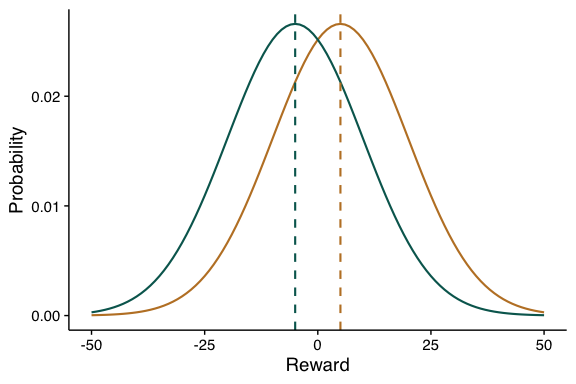
\includegraphics{hot_stove_sims_files/figure-latex/unnamed-chunk-9-1.pdf}

\begin{Shaded}
\begin{Highlighting}[]
\FunctionTok{ggplot}\NormalTok{(simsdf }\SpecialCharTok{\%\textgreater{}\%} \FunctionTok{filter}\NormalTok{(sim}\SpecialCharTok{\textless{}}\DecValTok{11}\NormalTok{) ,}\FunctionTok{aes}\NormalTok{(}\AttributeTok{x=}\NormalTok{trial, }\AttributeTok{group =}\NormalTok{ sim )) }\SpecialCharTok{+} 
 \FunctionTok{geom\_line}\NormalTok{(}\FunctionTok{aes}\NormalTok{(}\AttributeTok{y=}\NormalTok{estmu\_arm1),}\AttributeTok{color=}\NormalTok{hue\_arm1) }\SpecialCharTok{+} 
\FunctionTok{geom\_line}\NormalTok{(}\FunctionTok{aes}\NormalTok{(}\AttributeTok{y=}\NormalTok{estmu\_arm2),}\AttributeTok{color=}\NormalTok{hue\_arm2) }\SpecialCharTok{+} 
 \FunctionTok{geom\_hline}\NormalTok{(}\AttributeTok{yintercept =}\NormalTok{ mu\_arm1, }\AttributeTok{color=}\NormalTok{ hue\_arm1, }\AttributeTok{linetype=}\StringTok{"dashed"}\NormalTok{) }\SpecialCharTok{+} 
\FunctionTok{geom\_hline}\NormalTok{(}\AttributeTok{yintercept =}\NormalTok{ mu\_arm2, }\AttributeTok{color=}\NormalTok{ hue\_arm2, }\AttributeTok{linetype=}\StringTok{"dashed"}\NormalTok{) }\SpecialCharTok{+} 
\FunctionTok{facet\_wrap}\NormalTok{(}\SpecialCharTok{\textasciitilde{}}\NormalTok{tau) }\SpecialCharTok{+} 
\NormalTok{scalex\_trials }\SpecialCharTok{+}
\FunctionTok{ylab}\NormalTok{(}\StringTok{"Estimated value"}\NormalTok{) }\SpecialCharTok{+} 
\FunctionTok{theme}\NormalTok{(}\AttributeTok{strip.background =} \FunctionTok{element\_blank}\NormalTok{(), }\AttributeTok{strip.text.x =} \FunctionTok{element\_text}\NormalTok{(}\AttributeTok{face =} \StringTok{"bold"}\NormalTok{)) }\CommentTok{\#way to see a few blocks at the same time}
\end{Highlighting}
\end{Shaded}

\begin{verbatim}
## Warning: Removed 27 rows containing missing values (`geom_line()`).
\end{verbatim}

\begin{verbatim}
## Warning: Removed 16 rows containing missing values (`geom_line()`).
\end{verbatim}

\includegraphics{hot_stove_sims_files/figure-latex/unnamed-chunk-10-1.pdf}

\begin{Shaded}
\begin{Highlighting}[]
\FunctionTok{ggplot}\NormalTok{(sims\_sum\_df,}\FunctionTok{aes}\NormalTok{(}\AttributeTok{x=}\NormalTok{trial)) }\SpecialCharTok{+}
  \FunctionTok{geom\_ribbon}\NormalTok{(}\FunctionTok{aes}\NormalTok{(}\AttributeTok{ymin=}\NormalTok{choice\_arm1 }\SpecialCharTok{{-}}\NormalTok{ se\_choice\_arm1, }\AttributeTok{ymax=}\NormalTok{choice\_arm1 }\SpecialCharTok{+}\NormalTok{ se\_choice\_arm1,}\AttributeTok{fill=}\FunctionTok{as.factor}\NormalTok{(tau)),}\AttributeTok{alpha =} \FloatTok{0.25}\NormalTok{) }\SpecialCharTok{+}
  \FunctionTok{geom\_line}\NormalTok{(}\FunctionTok{aes}\NormalTok{(}\AttributeTok{y=}\NormalTok{choice\_arm1,}\AttributeTok{color=}\FunctionTok{as.factor}\NormalTok{(tau)),}\AttributeTok{size=}\DecValTok{1}\NormalTok{) }\SpecialCharTok{+} 
  \FunctionTok{ylim}\NormalTok{(}\FloatTok{0.4}\NormalTok{,}\FloatTok{0.9}\NormalTok{) }\SpecialCharTok{+} 
\NormalTok{  paltau\_color }\SpecialCharTok{+} 
\NormalTok{  paltau\_fill }\SpecialCharTok{+} 
\NormalTok{  scalex\_trials }\SpecialCharTok{+}
  \FunctionTok{ylab}\NormalTok{(}\StringTok{"Rate choices best a priori arm"}\NormalTok{) }\SpecialCharTok{+}
  \FunctionTok{theme}\NormalTok{(}
    \AttributeTok{legend.position =} \FunctionTok{c}\NormalTok{(}\FloatTok{0.75}\NormalTok{, }\FloatTok{0.1}\NormalTok{),}
    \AttributeTok{legend.direction =} \StringTok{"horizontal"}\NormalTok{)}
\end{Highlighting}
\end{Shaded}

\begin{verbatim}
## Warning in grid.Call(C_textBounds, as.graphicsAnnot(x$label), x$x, x$y, : font
## metrics unknown for Unicode character U+03c4

## Warning in grid.Call(C_textBounds, as.graphicsAnnot(x$label), x$x, x$y, : font
## metrics unknown for Unicode character U+03c4

## Warning in grid.Call(C_textBounds, as.graphicsAnnot(x$label), x$x, x$y, : font
## metrics unknown for Unicode character U+03c4

## Warning in grid.Call(C_textBounds, as.graphicsAnnot(x$label), x$x, x$y, : font
## metrics unknown for Unicode character U+03c4

## Warning in grid.Call(C_textBounds, as.graphicsAnnot(x$label), x$x, x$y, : font
## metrics unknown for Unicode character U+03c4

## Warning in grid.Call(C_textBounds, as.graphicsAnnot(x$label), x$x, x$y, : font
## metrics unknown for Unicode character U+03c4

## Warning in grid.Call(C_textBounds, as.graphicsAnnot(x$label), x$x, x$y, : font
## metrics unknown for Unicode character U+03c4

## Warning in grid.Call(C_textBounds, as.graphicsAnnot(x$label), x$x, x$y, : font
## metrics unknown for Unicode character U+03c4

## Warning in grid.Call(C_textBounds, as.graphicsAnnot(x$label), x$x, x$y, : font
## metrics unknown for Unicode character U+03c4

## Warning in grid.Call(C_textBounds, as.graphicsAnnot(x$label), x$x, x$y, : font
## metrics unknown for Unicode character U+03c4

## Warning in grid.Call(C_textBounds, as.graphicsAnnot(x$label), x$x, x$y, : font
## metrics unknown for Unicode character U+03c4

## Warning in grid.Call(C_textBounds, as.graphicsAnnot(x$label), x$x, x$y, : font
## metrics unknown for Unicode character U+03c4

## Warning in grid.Call(C_textBounds, as.graphicsAnnot(x$label), x$x, x$y, : font
## metrics unknown for Unicode character U+03c4

## Warning in grid.Call(C_textBounds, as.graphicsAnnot(x$label), x$x, x$y, : font
## metrics unknown for Unicode character U+03c4

## Warning in grid.Call(C_textBounds, as.graphicsAnnot(x$label), x$x, x$y, : font
## metrics unknown for Unicode character U+03c4

## Warning in grid.Call(C_textBounds, as.graphicsAnnot(x$label), x$x, x$y, : font
## metrics unknown for Unicode character U+03c4

## Warning in grid.Call(C_textBounds, as.graphicsAnnot(x$label), x$x, x$y, : font
## metrics unknown for Unicode character U+03c4

## Warning in grid.Call(C_textBounds, as.graphicsAnnot(x$label), x$x, x$y, : font
## metrics unknown for Unicode character U+03c4

## Warning in grid.Call(C_textBounds, as.graphicsAnnot(x$label), x$x, x$y, : font
## metrics unknown for Unicode character U+03c4

## Warning in grid.Call(C_textBounds, as.graphicsAnnot(x$label), x$x, x$y, : font
## metrics unknown for Unicode character U+03c4

## Warning in grid.Call(C_textBounds, as.graphicsAnnot(x$label), x$x, x$y, : font
## metrics unknown for Unicode character U+03c4

## Warning in grid.Call(C_textBounds, as.graphicsAnnot(x$label), x$x, x$y, : font
## metrics unknown for Unicode character U+03c4

## Warning in grid.Call(C_textBounds, as.graphicsAnnot(x$label), x$x, x$y, : font
## metrics unknown for Unicode character U+03c4

## Warning in grid.Call(C_textBounds, as.graphicsAnnot(x$label), x$x, x$y, : font
## metrics unknown for Unicode character U+03c4

## Warning in grid.Call(C_textBounds, as.graphicsAnnot(x$label), x$x, x$y, : font
## metrics unknown for Unicode character U+03c4

## Warning in grid.Call(C_textBounds, as.graphicsAnnot(x$label), x$x, x$y, : font
## metrics unknown for Unicode character U+03c4

## Warning in grid.Call(C_textBounds, as.graphicsAnnot(x$label), x$x, x$y, : font
## metrics unknown for Unicode character U+03c4

## Warning in grid.Call(C_textBounds, as.graphicsAnnot(x$label), x$x, x$y, : font
## metrics unknown for Unicode character U+03c4

## Warning in grid.Call(C_textBounds, as.graphicsAnnot(x$label), x$x, x$y, : font
## metrics unknown for Unicode character U+03c4

## Warning in grid.Call(C_textBounds, as.graphicsAnnot(x$label), x$x, x$y, : font
## metrics unknown for Unicode character U+03c4

## Warning in grid.Call(C_textBounds, as.graphicsAnnot(x$label), x$x, x$y, : font
## metrics unknown for Unicode character U+03c4

## Warning in grid.Call(C_textBounds, as.graphicsAnnot(x$label), x$x, x$y, : font
## metrics unknown for Unicode character U+03c4

## Warning in grid.Call(C_textBounds, as.graphicsAnnot(x$label), x$x, x$y, : font
## metrics unknown for Unicode character U+03c4

## Warning in grid.Call(C_textBounds, as.graphicsAnnot(x$label), x$x, x$y, : font
## metrics unknown for Unicode character U+03c4

## Warning in grid.Call(C_textBounds, as.graphicsAnnot(x$label), x$x, x$y, : font
## metrics unknown for Unicode character U+03c4

## Warning in grid.Call(C_textBounds, as.graphicsAnnot(x$label), x$x, x$y, : font
## metrics unknown for Unicode character U+03c4

## Warning in grid.Call(C_textBounds, as.graphicsAnnot(x$label), x$x, x$y, : font
## metrics unknown for Unicode character U+03c4

## Warning in grid.Call(C_textBounds, as.graphicsAnnot(x$label), x$x, x$y, : font
## metrics unknown for Unicode character U+03c4

## Warning in grid.Call(C_textBounds, as.graphicsAnnot(x$label), x$x, x$y, : font
## metrics unknown for Unicode character U+03c4

## Warning in grid.Call(C_textBounds, as.graphicsAnnot(x$label), x$x, x$y, : font
## metrics unknown for Unicode character U+03c4

## Warning in grid.Call(C_textBounds, as.graphicsAnnot(x$label), x$x, x$y, : font
## metrics unknown for Unicode character U+03c4

## Warning in grid.Call(C_textBounds, as.graphicsAnnot(x$label), x$x, x$y, : font
## metrics unknown for Unicode character U+03c4

## Warning in grid.Call(C_textBounds, as.graphicsAnnot(x$label), x$x, x$y, : font
## metrics unknown for Unicode character U+03c4

## Warning in grid.Call(C_textBounds, as.graphicsAnnot(x$label), x$x, x$y, : font
## metrics unknown for Unicode character U+03c4

## Warning in grid.Call(C_textBounds, as.graphicsAnnot(x$label), x$x, x$y, : font
## metrics unknown for Unicode character U+03c4

## Warning in grid.Call(C_textBounds, as.graphicsAnnot(x$label), x$x, x$y, : font
## metrics unknown for Unicode character U+03c4

## Warning in grid.Call(C_textBounds, as.graphicsAnnot(x$label), x$x, x$y, : font
## metrics unknown for Unicode character U+03c4

## Warning in grid.Call(C_textBounds, as.graphicsAnnot(x$label), x$x, x$y, : font
## metrics unknown for Unicode character U+03c4
\end{verbatim}

\begin{verbatim}
## Warning in grid.Call.graphics(C_text, as.graphicsAnnot(x$label), x$x, x$y, :
## font metrics unknown for Unicode character U+03c4

## Warning in grid.Call.graphics(C_text, as.graphicsAnnot(x$label), x$x, x$y, :
## font metrics unknown for Unicode character U+03c4
\end{verbatim}

\begin{verbatim}
## Warning in grid.Call.graphics(C_text, as.graphicsAnnot(x$label), x$x, x$y, :
## conversion failure on 'τ' in 'mbcsToSbcs': dot substituted for <cf>
\end{verbatim}

\begin{verbatim}
## Warning in grid.Call.graphics(C_text, as.graphicsAnnot(x$label), x$x, x$y, :
## conversion failure on 'τ' in 'mbcsToSbcs': dot substituted for <84>
\end{verbatim}

\includegraphics{hot_stove_sims_files/figure-latex/unnamed-chunk-11-1.pdf}

\begin{Shaded}
\begin{Highlighting}[]
\NormalTok{softm\_plot\_chobestapriori }\OtherTok{\textless{}{-}} \FunctionTok{ggplot}\NormalTok{(sims\_sum\_df,}\FunctionTok{aes}\NormalTok{(}\AttributeTok{x=}\NormalTok{trial)) }\SpecialCharTok{+}
  \FunctionTok{geom\_ribbon}\NormalTok{(}\FunctionTok{aes}\NormalTok{(}\AttributeTok{ymin=}\NormalTok{cum\_choice\_arm1 }\SpecialCharTok{{-}}\NormalTok{ se\_cum\_choice\_arm1, }\AttributeTok{ymax=}\NormalTok{cum\_choice\_arm1 }\SpecialCharTok{+}\NormalTok{ se\_cum\_choice\_arm1,}\AttributeTok{fill=}\FunctionTok{as.factor}\NormalTok{(tau)),}\AttributeTok{alpha =} \FloatTok{0.25}\NormalTok{) }\SpecialCharTok{+}
  \FunctionTok{geom\_line}\NormalTok{(}\FunctionTok{aes}\NormalTok{(}\AttributeTok{y=}\NormalTok{cum\_choice\_arm1,}\AttributeTok{color=}\FunctionTok{as.factor}\NormalTok{(tau)),}\AttributeTok{size=}\DecValTok{1}\NormalTok{) }\SpecialCharTok{+} 
  \FunctionTok{xlim}\NormalTok{(}\DecValTok{1}\NormalTok{,}\DecValTok{25}\NormalTok{) }\SpecialCharTok{+}
  \FunctionTok{ylim}\NormalTok{(}\FloatTok{0.4}\NormalTok{,}\FloatTok{0.9}\NormalTok{) }\SpecialCharTok{+} 
\NormalTok{  paltau\_color }\SpecialCharTok{+} 
\NormalTok{  paltau\_fill }\SpecialCharTok{+} 
\NormalTok{  scalex\_trials }\SpecialCharTok{+}
  \FunctionTok{ylab}\NormalTok{(}\StringTok{"Rate choices arm 1"}\NormalTok{) }\SpecialCharTok{+}
  \FunctionTok{theme}\NormalTok{(}
    \AttributeTok{legend.position =} \FunctionTok{c}\NormalTok{(}\FloatTok{0.75}\NormalTok{, }\FloatTok{0.1}\NormalTok{),}
    \AttributeTok{legend.direction =} \StringTok{"horizontal"}\NormalTok{)}
\end{Highlighting}
\end{Shaded}

\begin{verbatim}
## Scale for x is already present.
## Adding another scale for x, which will replace the existing scale.
\end{verbatim}

\begin{Shaded}
\begin{Highlighting}[]
\NormalTok{softm\_plot\_chobestapriori}
\end{Highlighting}
\end{Shaded}

\begin{verbatim}
## Warning in grid.Call(C_textBounds, as.graphicsAnnot(x$label), x$x, x$y, : font
## metrics unknown for Unicode character U+03c4

## Warning in grid.Call(C_textBounds, as.graphicsAnnot(x$label), x$x, x$y, : font
## metrics unknown for Unicode character U+03c4

## Warning in grid.Call(C_textBounds, as.graphicsAnnot(x$label), x$x, x$y, : font
## metrics unknown for Unicode character U+03c4

## Warning in grid.Call(C_textBounds, as.graphicsAnnot(x$label), x$x, x$y, : font
## metrics unknown for Unicode character U+03c4

## Warning in grid.Call(C_textBounds, as.graphicsAnnot(x$label), x$x, x$y, : font
## metrics unknown for Unicode character U+03c4

## Warning in grid.Call(C_textBounds, as.graphicsAnnot(x$label), x$x, x$y, : font
## metrics unknown for Unicode character U+03c4

## Warning in grid.Call(C_textBounds, as.graphicsAnnot(x$label), x$x, x$y, : font
## metrics unknown for Unicode character U+03c4

## Warning in grid.Call(C_textBounds, as.graphicsAnnot(x$label), x$x, x$y, : font
## metrics unknown for Unicode character U+03c4

## Warning in grid.Call(C_textBounds, as.graphicsAnnot(x$label), x$x, x$y, : font
## metrics unknown for Unicode character U+03c4

## Warning in grid.Call(C_textBounds, as.graphicsAnnot(x$label), x$x, x$y, : font
## metrics unknown for Unicode character U+03c4

## Warning in grid.Call(C_textBounds, as.graphicsAnnot(x$label), x$x, x$y, : font
## metrics unknown for Unicode character U+03c4

## Warning in grid.Call(C_textBounds, as.graphicsAnnot(x$label), x$x, x$y, : font
## metrics unknown for Unicode character U+03c4

## Warning in grid.Call(C_textBounds, as.graphicsAnnot(x$label), x$x, x$y, : font
## metrics unknown for Unicode character U+03c4

## Warning in grid.Call(C_textBounds, as.graphicsAnnot(x$label), x$x, x$y, : font
## metrics unknown for Unicode character U+03c4

## Warning in grid.Call(C_textBounds, as.graphicsAnnot(x$label), x$x, x$y, : font
## metrics unknown for Unicode character U+03c4

## Warning in grid.Call(C_textBounds, as.graphicsAnnot(x$label), x$x, x$y, : font
## metrics unknown for Unicode character U+03c4

## Warning in grid.Call(C_textBounds, as.graphicsAnnot(x$label), x$x, x$y, : font
## metrics unknown for Unicode character U+03c4

## Warning in grid.Call(C_textBounds, as.graphicsAnnot(x$label), x$x, x$y, : font
## metrics unknown for Unicode character U+03c4

## Warning in grid.Call(C_textBounds, as.graphicsAnnot(x$label), x$x, x$y, : font
## metrics unknown for Unicode character U+03c4

## Warning in grid.Call(C_textBounds, as.graphicsAnnot(x$label), x$x, x$y, : font
## metrics unknown for Unicode character U+03c4

## Warning in grid.Call(C_textBounds, as.graphicsAnnot(x$label), x$x, x$y, : font
## metrics unknown for Unicode character U+03c4

## Warning in grid.Call(C_textBounds, as.graphicsAnnot(x$label), x$x, x$y, : font
## metrics unknown for Unicode character U+03c4

## Warning in grid.Call(C_textBounds, as.graphicsAnnot(x$label), x$x, x$y, : font
## metrics unknown for Unicode character U+03c4

## Warning in grid.Call(C_textBounds, as.graphicsAnnot(x$label), x$x, x$y, : font
## metrics unknown for Unicode character U+03c4

## Warning in grid.Call(C_textBounds, as.graphicsAnnot(x$label), x$x, x$y, : font
## metrics unknown for Unicode character U+03c4

## Warning in grid.Call(C_textBounds, as.graphicsAnnot(x$label), x$x, x$y, : font
## metrics unknown for Unicode character U+03c4

## Warning in grid.Call(C_textBounds, as.graphicsAnnot(x$label), x$x, x$y, : font
## metrics unknown for Unicode character U+03c4

## Warning in grid.Call(C_textBounds, as.graphicsAnnot(x$label), x$x, x$y, : font
## metrics unknown for Unicode character U+03c4

## Warning in grid.Call(C_textBounds, as.graphicsAnnot(x$label), x$x, x$y, : font
## metrics unknown for Unicode character U+03c4

## Warning in grid.Call(C_textBounds, as.graphicsAnnot(x$label), x$x, x$y, : font
## metrics unknown for Unicode character U+03c4

## Warning in grid.Call(C_textBounds, as.graphicsAnnot(x$label), x$x, x$y, : font
## metrics unknown for Unicode character U+03c4

## Warning in grid.Call(C_textBounds, as.graphicsAnnot(x$label), x$x, x$y, : font
## metrics unknown for Unicode character U+03c4

## Warning in grid.Call(C_textBounds, as.graphicsAnnot(x$label), x$x, x$y, : font
## metrics unknown for Unicode character U+03c4

## Warning in grid.Call(C_textBounds, as.graphicsAnnot(x$label), x$x, x$y, : font
## metrics unknown for Unicode character U+03c4

## Warning in grid.Call(C_textBounds, as.graphicsAnnot(x$label), x$x, x$y, : font
## metrics unknown for Unicode character U+03c4

## Warning in grid.Call(C_textBounds, as.graphicsAnnot(x$label), x$x, x$y, : font
## metrics unknown for Unicode character U+03c4

## Warning in grid.Call(C_textBounds, as.graphicsAnnot(x$label), x$x, x$y, : font
## metrics unknown for Unicode character U+03c4

## Warning in grid.Call(C_textBounds, as.graphicsAnnot(x$label), x$x, x$y, : font
## metrics unknown for Unicode character U+03c4

## Warning in grid.Call(C_textBounds, as.graphicsAnnot(x$label), x$x, x$y, : font
## metrics unknown for Unicode character U+03c4

## Warning in grid.Call(C_textBounds, as.graphicsAnnot(x$label), x$x, x$y, : font
## metrics unknown for Unicode character U+03c4

## Warning in grid.Call(C_textBounds, as.graphicsAnnot(x$label), x$x, x$y, : font
## metrics unknown for Unicode character U+03c4

## Warning in grid.Call(C_textBounds, as.graphicsAnnot(x$label), x$x, x$y, : font
## metrics unknown for Unicode character U+03c4

## Warning in grid.Call(C_textBounds, as.graphicsAnnot(x$label), x$x, x$y, : font
## metrics unknown for Unicode character U+03c4

## Warning in grid.Call(C_textBounds, as.graphicsAnnot(x$label), x$x, x$y, : font
## metrics unknown for Unicode character U+03c4

## Warning in grid.Call(C_textBounds, as.graphicsAnnot(x$label), x$x, x$y, : font
## metrics unknown for Unicode character U+03c4

## Warning in grid.Call(C_textBounds, as.graphicsAnnot(x$label), x$x, x$y, : font
## metrics unknown for Unicode character U+03c4

## Warning in grid.Call(C_textBounds, as.graphicsAnnot(x$label), x$x, x$y, : font
## metrics unknown for Unicode character U+03c4

## Warning in grid.Call(C_textBounds, as.graphicsAnnot(x$label), x$x, x$y, : font
## metrics unknown for Unicode character U+03c4
\end{verbatim}

\begin{verbatim}
## Warning in grid.Call.graphics(C_text, as.graphicsAnnot(x$label), x$x, x$y, :
## font metrics unknown for Unicode character U+03c4

## Warning in grid.Call.graphics(C_text, as.graphicsAnnot(x$label), x$x, x$y, :
## font metrics unknown for Unicode character U+03c4
\end{verbatim}

\begin{verbatim}
## Warning in grid.Call.graphics(C_text, as.graphicsAnnot(x$label), x$x, x$y, :
## conversion failure on 'τ' in 'mbcsToSbcs': dot substituted for <cf>
\end{verbatim}

\begin{verbatim}
## Warning in grid.Call.graphics(C_text, as.graphicsAnnot(x$label), x$x, x$y, :
## conversion failure on 'τ' in 'mbcsToSbcs': dot substituted for <84>
\end{verbatim}

\includegraphics{hot_stove_sims_files/figure-latex/unnamed-chunk-12-1.pdf}

\begin{Shaded}
\begin{Highlighting}[]
\NormalTok{softm\_plot\_chobestobs }\OtherTok{\textless{}{-}} \FunctionTok{ggplot}\NormalTok{(sims\_sum\_df,}\FunctionTok{aes}\NormalTok{(}\AttributeTok{x=}\NormalTok{trial)) }\SpecialCharTok{+} 
  \FunctionTok{geom\_ribbon}\NormalTok{(}\FunctionTok{aes}\NormalTok{(}\AttributeTok{ymin=}\NormalTok{choice\_bestobsrewarm }\SpecialCharTok{{-}}\NormalTok{ se\_choice\_bestobsrewarm, }\AttributeTok{ymax=}\NormalTok{choice\_bestobsrewarm }\SpecialCharTok{+}\NormalTok{ se\_choice\_bestobsrewarm,}\AttributeTok{fill=}\FunctionTok{as.factor}\NormalTok{(tau)),}\AttributeTok{alpha =} \FloatTok{0.25}\NormalTok{) }\SpecialCharTok{+}
  \FunctionTok{geom\_line}\NormalTok{(}\FunctionTok{aes}\NormalTok{(}\AttributeTok{y=}\NormalTok{choice\_bestobsrewarm,}\AttributeTok{color=}\FunctionTok{as.factor}\NormalTok{(tau)),}\AttributeTok{size=}\DecValTok{1}\NormalTok{) }\SpecialCharTok{+}
  \FunctionTok{ylim}\NormalTok{(}\FloatTok{0.4}\NormalTok{,}\FloatTok{0.9}\NormalTok{) }\SpecialCharTok{+} 
\NormalTok{  paltau\_color }\SpecialCharTok{+} 
\NormalTok{  paltau\_fill }\SpecialCharTok{+} 
\NormalTok{  scalex\_trials }\SpecialCharTok{+}
  \FunctionTok{ylab}\NormalTok{(}\StringTok{"Rate choices best observed arm"}\NormalTok{) }\SpecialCharTok{+}
  \FunctionTok{theme}\NormalTok{(}
    \AttributeTok{legend.position =} \FunctionTok{c}\NormalTok{(}\FloatTok{0.75}\NormalTok{, }\FloatTok{0.1}\NormalTok{),}
    \AttributeTok{legend.direction =} \StringTok{"horizontal"}\NormalTok{)}

\NormalTok{softm\_plot\_chobestobs}
\end{Highlighting}
\end{Shaded}

\begin{verbatim}
## Warning: Removed 4 rows containing missing values (`geom_line()`).
\end{verbatim}

\begin{verbatim}
## Warning in grid.Call(C_textBounds, as.graphicsAnnot(x$label), x$x, x$y, : font
## metrics unknown for Unicode character U+03c4

## Warning in grid.Call(C_textBounds, as.graphicsAnnot(x$label), x$x, x$y, : font
## metrics unknown for Unicode character U+03c4

## Warning in grid.Call(C_textBounds, as.graphicsAnnot(x$label), x$x, x$y, : font
## metrics unknown for Unicode character U+03c4

## Warning in grid.Call(C_textBounds, as.graphicsAnnot(x$label), x$x, x$y, : font
## metrics unknown for Unicode character U+03c4

## Warning in grid.Call(C_textBounds, as.graphicsAnnot(x$label), x$x, x$y, : font
## metrics unknown for Unicode character U+03c4

## Warning in grid.Call(C_textBounds, as.graphicsAnnot(x$label), x$x, x$y, : font
## metrics unknown for Unicode character U+03c4

## Warning in grid.Call(C_textBounds, as.graphicsAnnot(x$label), x$x, x$y, : font
## metrics unknown for Unicode character U+03c4

## Warning in grid.Call(C_textBounds, as.graphicsAnnot(x$label), x$x, x$y, : font
## metrics unknown for Unicode character U+03c4

## Warning in grid.Call(C_textBounds, as.graphicsAnnot(x$label), x$x, x$y, : font
## metrics unknown for Unicode character U+03c4

## Warning in grid.Call(C_textBounds, as.graphicsAnnot(x$label), x$x, x$y, : font
## metrics unknown for Unicode character U+03c4

## Warning in grid.Call(C_textBounds, as.graphicsAnnot(x$label), x$x, x$y, : font
## metrics unknown for Unicode character U+03c4

## Warning in grid.Call(C_textBounds, as.graphicsAnnot(x$label), x$x, x$y, : font
## metrics unknown for Unicode character U+03c4

## Warning in grid.Call(C_textBounds, as.graphicsAnnot(x$label), x$x, x$y, : font
## metrics unknown for Unicode character U+03c4

## Warning in grid.Call(C_textBounds, as.graphicsAnnot(x$label), x$x, x$y, : font
## metrics unknown for Unicode character U+03c4

## Warning in grid.Call(C_textBounds, as.graphicsAnnot(x$label), x$x, x$y, : font
## metrics unknown for Unicode character U+03c4

## Warning in grid.Call(C_textBounds, as.graphicsAnnot(x$label), x$x, x$y, : font
## metrics unknown for Unicode character U+03c4

## Warning in grid.Call(C_textBounds, as.graphicsAnnot(x$label), x$x, x$y, : font
## metrics unknown for Unicode character U+03c4

## Warning in grid.Call(C_textBounds, as.graphicsAnnot(x$label), x$x, x$y, : font
## metrics unknown for Unicode character U+03c4

## Warning in grid.Call(C_textBounds, as.graphicsAnnot(x$label), x$x, x$y, : font
## metrics unknown for Unicode character U+03c4

## Warning in grid.Call(C_textBounds, as.graphicsAnnot(x$label), x$x, x$y, : font
## metrics unknown for Unicode character U+03c4

## Warning in grid.Call(C_textBounds, as.graphicsAnnot(x$label), x$x, x$y, : font
## metrics unknown for Unicode character U+03c4

## Warning in grid.Call(C_textBounds, as.graphicsAnnot(x$label), x$x, x$y, : font
## metrics unknown for Unicode character U+03c4

## Warning in grid.Call(C_textBounds, as.graphicsAnnot(x$label), x$x, x$y, : font
## metrics unknown for Unicode character U+03c4

## Warning in grid.Call(C_textBounds, as.graphicsAnnot(x$label), x$x, x$y, : font
## metrics unknown for Unicode character U+03c4

## Warning in grid.Call(C_textBounds, as.graphicsAnnot(x$label), x$x, x$y, : font
## metrics unknown for Unicode character U+03c4

## Warning in grid.Call(C_textBounds, as.graphicsAnnot(x$label), x$x, x$y, : font
## metrics unknown for Unicode character U+03c4

## Warning in grid.Call(C_textBounds, as.graphicsAnnot(x$label), x$x, x$y, : font
## metrics unknown for Unicode character U+03c4

## Warning in grid.Call(C_textBounds, as.graphicsAnnot(x$label), x$x, x$y, : font
## metrics unknown for Unicode character U+03c4

## Warning in grid.Call(C_textBounds, as.graphicsAnnot(x$label), x$x, x$y, : font
## metrics unknown for Unicode character U+03c4

## Warning in grid.Call(C_textBounds, as.graphicsAnnot(x$label), x$x, x$y, : font
## metrics unknown for Unicode character U+03c4

## Warning in grid.Call(C_textBounds, as.graphicsAnnot(x$label), x$x, x$y, : font
## metrics unknown for Unicode character U+03c4

## Warning in grid.Call(C_textBounds, as.graphicsAnnot(x$label), x$x, x$y, : font
## metrics unknown for Unicode character U+03c4

## Warning in grid.Call(C_textBounds, as.graphicsAnnot(x$label), x$x, x$y, : font
## metrics unknown for Unicode character U+03c4

## Warning in grid.Call(C_textBounds, as.graphicsAnnot(x$label), x$x, x$y, : font
## metrics unknown for Unicode character U+03c4

## Warning in grid.Call(C_textBounds, as.graphicsAnnot(x$label), x$x, x$y, : font
## metrics unknown for Unicode character U+03c4

## Warning in grid.Call(C_textBounds, as.graphicsAnnot(x$label), x$x, x$y, : font
## metrics unknown for Unicode character U+03c4

## Warning in grid.Call(C_textBounds, as.graphicsAnnot(x$label), x$x, x$y, : font
## metrics unknown for Unicode character U+03c4

## Warning in grid.Call(C_textBounds, as.graphicsAnnot(x$label), x$x, x$y, : font
## metrics unknown for Unicode character U+03c4

## Warning in grid.Call(C_textBounds, as.graphicsAnnot(x$label), x$x, x$y, : font
## metrics unknown for Unicode character U+03c4

## Warning in grid.Call(C_textBounds, as.graphicsAnnot(x$label), x$x, x$y, : font
## metrics unknown for Unicode character U+03c4

## Warning in grid.Call(C_textBounds, as.graphicsAnnot(x$label), x$x, x$y, : font
## metrics unknown for Unicode character U+03c4

## Warning in grid.Call(C_textBounds, as.graphicsAnnot(x$label), x$x, x$y, : font
## metrics unknown for Unicode character U+03c4

## Warning in grid.Call(C_textBounds, as.graphicsAnnot(x$label), x$x, x$y, : font
## metrics unknown for Unicode character U+03c4

## Warning in grid.Call(C_textBounds, as.graphicsAnnot(x$label), x$x, x$y, : font
## metrics unknown for Unicode character U+03c4

## Warning in grid.Call(C_textBounds, as.graphicsAnnot(x$label), x$x, x$y, : font
## metrics unknown for Unicode character U+03c4

## Warning in grid.Call(C_textBounds, as.graphicsAnnot(x$label), x$x, x$y, : font
## metrics unknown for Unicode character U+03c4

## Warning in grid.Call(C_textBounds, as.graphicsAnnot(x$label), x$x, x$y, : font
## metrics unknown for Unicode character U+03c4

## Warning in grid.Call(C_textBounds, as.graphicsAnnot(x$label), x$x, x$y, : font
## metrics unknown for Unicode character U+03c4
\end{verbatim}

\begin{verbatim}
## Warning in grid.Call.graphics(C_text, as.graphicsAnnot(x$label), x$x, x$y, :
## font metrics unknown for Unicode character U+03c4

## Warning in grid.Call.graphics(C_text, as.graphicsAnnot(x$label), x$x, x$y, :
## font metrics unknown for Unicode character U+03c4
\end{verbatim}

\begin{verbatim}
## Warning in grid.Call.graphics(C_text, as.graphicsAnnot(x$label), x$x, x$y, :
## conversion failure on 'τ' in 'mbcsToSbcs': dot substituted for <cf>
\end{verbatim}

\begin{verbatim}
## Warning in grid.Call.graphics(C_text, as.graphicsAnnot(x$label), x$x, x$y, :
## conversion failure on 'τ' in 'mbcsToSbcs': dot substituted for <84>
\end{verbatim}

\includegraphics{hot_stove_sims_files/figure-latex/unnamed-chunk-13-1.pdf}

\begin{Shaded}
\begin{Highlighting}[]
\NormalTok{softm\_plot\_exploit }\OtherTok{\textless{}{-}} \FunctionTok{ggplot}\NormalTok{(sims\_sum\_df,}\FunctionTok{aes}\NormalTok{(}\AttributeTok{x=}\NormalTok{trial)) }\SpecialCharTok{+} 
  \FunctionTok{geom\_ribbon}\NormalTok{(}\FunctionTok{aes}\NormalTok{(}\AttributeTok{ymin=}\NormalTok{exploit\_choice }\SpecialCharTok{{-}}\NormalTok{ se\_exploit\_choice, }\AttributeTok{ymax=}\NormalTok{exploit\_choice }\SpecialCharTok{+}\NormalTok{ se\_exploit\_choice,}\AttributeTok{fill=}\FunctionTok{as.factor}\NormalTok{(tau)),}\AttributeTok{alpha =} \FloatTok{0.25}\NormalTok{) }\SpecialCharTok{+}
  \FunctionTok{geom\_line}\NormalTok{(}\FunctionTok{aes}\NormalTok{(}\AttributeTok{y=}\NormalTok{exploit\_choice,}\AttributeTok{color=}\FunctionTok{as.factor}\NormalTok{(tau)),}\AttributeTok{size=}\DecValTok{1}\NormalTok{) }\SpecialCharTok{+}
  \CommentTok{\#ylim(0.4,0.9) + }
\NormalTok{  paltau\_color }\SpecialCharTok{+} 
\NormalTok{  paltau\_fill }\SpecialCharTok{+} 
\NormalTok{  scalex\_trials }\SpecialCharTok{+}
  \FunctionTok{ylab}\NormalTok{(}\StringTok{"Rate of exploitation choices"}\NormalTok{) }\SpecialCharTok{+}
  \FunctionTok{theme}\NormalTok{(}
    \AttributeTok{legend.position =} \FunctionTok{c}\NormalTok{(}\FloatTok{0.75}\NormalTok{, }\FloatTok{0.7}\NormalTok{),}
    \AttributeTok{legend.direction =} \StringTok{"horizontal"}\NormalTok{)}

\NormalTok{softm\_plot\_exploit}
\end{Highlighting}
\end{Shaded}

\begin{verbatim}
## Warning: Removed 8 rows containing missing values (`geom_line()`).
\end{verbatim}

\begin{verbatim}
## Warning in grid.Call(C_textBounds, as.graphicsAnnot(x$label), x$x, x$y, : font
## metrics unknown for Unicode character U+03c4

## Warning in grid.Call(C_textBounds, as.graphicsAnnot(x$label), x$x, x$y, : font
## metrics unknown for Unicode character U+03c4

## Warning in grid.Call(C_textBounds, as.graphicsAnnot(x$label), x$x, x$y, : font
## metrics unknown for Unicode character U+03c4

## Warning in grid.Call(C_textBounds, as.graphicsAnnot(x$label), x$x, x$y, : font
## metrics unknown for Unicode character U+03c4

## Warning in grid.Call(C_textBounds, as.graphicsAnnot(x$label), x$x, x$y, : font
## metrics unknown for Unicode character U+03c4

## Warning in grid.Call(C_textBounds, as.graphicsAnnot(x$label), x$x, x$y, : font
## metrics unknown for Unicode character U+03c4

## Warning in grid.Call(C_textBounds, as.graphicsAnnot(x$label), x$x, x$y, : font
## metrics unknown for Unicode character U+03c4

## Warning in grid.Call(C_textBounds, as.graphicsAnnot(x$label), x$x, x$y, : font
## metrics unknown for Unicode character U+03c4

## Warning in grid.Call(C_textBounds, as.graphicsAnnot(x$label), x$x, x$y, : font
## metrics unknown for Unicode character U+03c4

## Warning in grid.Call(C_textBounds, as.graphicsAnnot(x$label), x$x, x$y, : font
## metrics unknown for Unicode character U+03c4

## Warning in grid.Call(C_textBounds, as.graphicsAnnot(x$label), x$x, x$y, : font
## metrics unknown for Unicode character U+03c4

## Warning in grid.Call(C_textBounds, as.graphicsAnnot(x$label), x$x, x$y, : font
## metrics unknown for Unicode character U+03c4

## Warning in grid.Call(C_textBounds, as.graphicsAnnot(x$label), x$x, x$y, : font
## metrics unknown for Unicode character U+03c4

## Warning in grid.Call(C_textBounds, as.graphicsAnnot(x$label), x$x, x$y, : font
## metrics unknown for Unicode character U+03c4

## Warning in grid.Call(C_textBounds, as.graphicsAnnot(x$label), x$x, x$y, : font
## metrics unknown for Unicode character U+03c4

## Warning in grid.Call(C_textBounds, as.graphicsAnnot(x$label), x$x, x$y, : font
## metrics unknown for Unicode character U+03c4

## Warning in grid.Call(C_textBounds, as.graphicsAnnot(x$label), x$x, x$y, : font
## metrics unknown for Unicode character U+03c4

## Warning in grid.Call(C_textBounds, as.graphicsAnnot(x$label), x$x, x$y, : font
## metrics unknown for Unicode character U+03c4

## Warning in grid.Call(C_textBounds, as.graphicsAnnot(x$label), x$x, x$y, : font
## metrics unknown for Unicode character U+03c4

## Warning in grid.Call(C_textBounds, as.graphicsAnnot(x$label), x$x, x$y, : font
## metrics unknown for Unicode character U+03c4

## Warning in grid.Call(C_textBounds, as.graphicsAnnot(x$label), x$x, x$y, : font
## metrics unknown for Unicode character U+03c4

## Warning in grid.Call(C_textBounds, as.graphicsAnnot(x$label), x$x, x$y, : font
## metrics unknown for Unicode character U+03c4

## Warning in grid.Call(C_textBounds, as.graphicsAnnot(x$label), x$x, x$y, : font
## metrics unknown for Unicode character U+03c4

## Warning in grid.Call(C_textBounds, as.graphicsAnnot(x$label), x$x, x$y, : font
## metrics unknown for Unicode character U+03c4

## Warning in grid.Call(C_textBounds, as.graphicsAnnot(x$label), x$x, x$y, : font
## metrics unknown for Unicode character U+03c4

## Warning in grid.Call(C_textBounds, as.graphicsAnnot(x$label), x$x, x$y, : font
## metrics unknown for Unicode character U+03c4

## Warning in grid.Call(C_textBounds, as.graphicsAnnot(x$label), x$x, x$y, : font
## metrics unknown for Unicode character U+03c4

## Warning in grid.Call(C_textBounds, as.graphicsAnnot(x$label), x$x, x$y, : font
## metrics unknown for Unicode character U+03c4

## Warning in grid.Call(C_textBounds, as.graphicsAnnot(x$label), x$x, x$y, : font
## metrics unknown for Unicode character U+03c4

## Warning in grid.Call(C_textBounds, as.graphicsAnnot(x$label), x$x, x$y, : font
## metrics unknown for Unicode character U+03c4

## Warning in grid.Call(C_textBounds, as.graphicsAnnot(x$label), x$x, x$y, : font
## metrics unknown for Unicode character U+03c4

## Warning in grid.Call(C_textBounds, as.graphicsAnnot(x$label), x$x, x$y, : font
## metrics unknown for Unicode character U+03c4

## Warning in grid.Call(C_textBounds, as.graphicsAnnot(x$label), x$x, x$y, : font
## metrics unknown for Unicode character U+03c4

## Warning in grid.Call(C_textBounds, as.graphicsAnnot(x$label), x$x, x$y, : font
## metrics unknown for Unicode character U+03c4

## Warning in grid.Call(C_textBounds, as.graphicsAnnot(x$label), x$x, x$y, : font
## metrics unknown for Unicode character U+03c4

## Warning in grid.Call(C_textBounds, as.graphicsAnnot(x$label), x$x, x$y, : font
## metrics unknown for Unicode character U+03c4

## Warning in grid.Call(C_textBounds, as.graphicsAnnot(x$label), x$x, x$y, : font
## metrics unknown for Unicode character U+03c4

## Warning in grid.Call(C_textBounds, as.graphicsAnnot(x$label), x$x, x$y, : font
## metrics unknown for Unicode character U+03c4

## Warning in grid.Call(C_textBounds, as.graphicsAnnot(x$label), x$x, x$y, : font
## metrics unknown for Unicode character U+03c4

## Warning in grid.Call(C_textBounds, as.graphicsAnnot(x$label), x$x, x$y, : font
## metrics unknown for Unicode character U+03c4

## Warning in grid.Call(C_textBounds, as.graphicsAnnot(x$label), x$x, x$y, : font
## metrics unknown for Unicode character U+03c4

## Warning in grid.Call(C_textBounds, as.graphicsAnnot(x$label), x$x, x$y, : font
## metrics unknown for Unicode character U+03c4

## Warning in grid.Call(C_textBounds, as.graphicsAnnot(x$label), x$x, x$y, : font
## metrics unknown for Unicode character U+03c4

## Warning in grid.Call(C_textBounds, as.graphicsAnnot(x$label), x$x, x$y, : font
## metrics unknown for Unicode character U+03c4

## Warning in grid.Call(C_textBounds, as.graphicsAnnot(x$label), x$x, x$y, : font
## metrics unknown for Unicode character U+03c4

## Warning in grid.Call(C_textBounds, as.graphicsAnnot(x$label), x$x, x$y, : font
## metrics unknown for Unicode character U+03c4

## Warning in grid.Call(C_textBounds, as.graphicsAnnot(x$label), x$x, x$y, : font
## metrics unknown for Unicode character U+03c4

## Warning in grid.Call(C_textBounds, as.graphicsAnnot(x$label), x$x, x$y, : font
## metrics unknown for Unicode character U+03c4
\end{verbatim}

\begin{verbatim}
## Warning in grid.Call.graphics(C_text, as.graphicsAnnot(x$label), x$x, x$y, :
## font metrics unknown for Unicode character U+03c4

## Warning in grid.Call.graphics(C_text, as.graphicsAnnot(x$label), x$x, x$y, :
## font metrics unknown for Unicode character U+03c4
\end{verbatim}

\begin{verbatim}
## Warning in grid.Call.graphics(C_text, as.graphicsAnnot(x$label), x$x, x$y, :
## conversion failure on 'τ' in 'mbcsToSbcs': dot substituted for <cf>
\end{verbatim}

\begin{verbatim}
## Warning in grid.Call.graphics(C_text, as.graphicsAnnot(x$label), x$x, x$y, :
## conversion failure on 'τ' in 'mbcsToSbcs': dot substituted for <84>
\end{verbatim}

\includegraphics{hot_stove_sims_files/figure-latex/unnamed-chunk-14-1.pdf}

\begin{Shaded}
\begin{Highlighting}[]
\NormalTok{softm\_plot\_cumrew }\OtherTok{\textless{}{-}}\FunctionTok{ggplot}\NormalTok{(sims\_sum\_df,}\FunctionTok{aes}\NormalTok{(}\AttributeTok{x=}\NormalTok{trial)) }\SpecialCharTok{+} 
  \FunctionTok{geom\_ribbon}\NormalTok{(}\FunctionTok{aes}\NormalTok{(}\AttributeTok{ymin=}\NormalTok{cumrew }\SpecialCharTok{{-}}\NormalTok{ se\_cumrew, }\AttributeTok{ymax=}\NormalTok{cumrew }\SpecialCharTok{+}\NormalTok{ se\_cumrew,}\AttributeTok{fill=}\FunctionTok{as.factor}\NormalTok{(tau)),}\AttributeTok{alpha =} \FloatTok{0.25}\NormalTok{) }\SpecialCharTok{+}
  \FunctionTok{geom\_line}\NormalTok{(}\FunctionTok{aes}\NormalTok{(}\AttributeTok{y=}\NormalTok{cumrew,}\AttributeTok{color=}\FunctionTok{as.factor}\NormalTok{(tau)),}\AttributeTok{size=}\DecValTok{1}\NormalTok{) }\SpecialCharTok{+} 
\NormalTok{  paltau\_color }\SpecialCharTok{+} 
\NormalTok{  paltau\_fill }\SpecialCharTok{+} 
\NormalTok{  scalex\_trials }\SpecialCharTok{+}
  \FunctionTok{ylab}\NormalTok{(}\StringTok{"Cumulative reward"}\NormalTok{) }\SpecialCharTok{+}
  \FunctionTok{theme}\NormalTok{(}
    \AttributeTok{legend.position =} \FunctionTok{c}\NormalTok{(}\FloatTok{0.75}\NormalTok{, }\FloatTok{0.1}\NormalTok{),}
    \AttributeTok{legend.direction =} \StringTok{"horizontal"}\NormalTok{)}

\NormalTok{softm\_plot\_cumrew}
\end{Highlighting}
\end{Shaded}

\begin{verbatim}
## Warning in grid.Call(C_textBounds, as.graphicsAnnot(x$label), x$x, x$y, : font
## metrics unknown for Unicode character U+03c4

## Warning in grid.Call(C_textBounds, as.graphicsAnnot(x$label), x$x, x$y, : font
## metrics unknown for Unicode character U+03c4

## Warning in grid.Call(C_textBounds, as.graphicsAnnot(x$label), x$x, x$y, : font
## metrics unknown for Unicode character U+03c4

## Warning in grid.Call(C_textBounds, as.graphicsAnnot(x$label), x$x, x$y, : font
## metrics unknown for Unicode character U+03c4

## Warning in grid.Call(C_textBounds, as.graphicsAnnot(x$label), x$x, x$y, : font
## metrics unknown for Unicode character U+03c4

## Warning in grid.Call(C_textBounds, as.graphicsAnnot(x$label), x$x, x$y, : font
## metrics unknown for Unicode character U+03c4

## Warning in grid.Call(C_textBounds, as.graphicsAnnot(x$label), x$x, x$y, : font
## metrics unknown for Unicode character U+03c4

## Warning in grid.Call(C_textBounds, as.graphicsAnnot(x$label), x$x, x$y, : font
## metrics unknown for Unicode character U+03c4

## Warning in grid.Call(C_textBounds, as.graphicsAnnot(x$label), x$x, x$y, : font
## metrics unknown for Unicode character U+03c4

## Warning in grid.Call(C_textBounds, as.graphicsAnnot(x$label), x$x, x$y, : font
## metrics unknown for Unicode character U+03c4

## Warning in grid.Call(C_textBounds, as.graphicsAnnot(x$label), x$x, x$y, : font
## metrics unknown for Unicode character U+03c4

## Warning in grid.Call(C_textBounds, as.graphicsAnnot(x$label), x$x, x$y, : font
## metrics unknown for Unicode character U+03c4

## Warning in grid.Call(C_textBounds, as.graphicsAnnot(x$label), x$x, x$y, : font
## metrics unknown for Unicode character U+03c4

## Warning in grid.Call(C_textBounds, as.graphicsAnnot(x$label), x$x, x$y, : font
## metrics unknown for Unicode character U+03c4

## Warning in grid.Call(C_textBounds, as.graphicsAnnot(x$label), x$x, x$y, : font
## metrics unknown for Unicode character U+03c4

## Warning in grid.Call(C_textBounds, as.graphicsAnnot(x$label), x$x, x$y, : font
## metrics unknown for Unicode character U+03c4

## Warning in grid.Call(C_textBounds, as.graphicsAnnot(x$label), x$x, x$y, : font
## metrics unknown for Unicode character U+03c4

## Warning in grid.Call(C_textBounds, as.graphicsAnnot(x$label), x$x, x$y, : font
## metrics unknown for Unicode character U+03c4

## Warning in grid.Call(C_textBounds, as.graphicsAnnot(x$label), x$x, x$y, : font
## metrics unknown for Unicode character U+03c4

## Warning in grid.Call(C_textBounds, as.graphicsAnnot(x$label), x$x, x$y, : font
## metrics unknown for Unicode character U+03c4

## Warning in grid.Call(C_textBounds, as.graphicsAnnot(x$label), x$x, x$y, : font
## metrics unknown for Unicode character U+03c4

## Warning in grid.Call(C_textBounds, as.graphicsAnnot(x$label), x$x, x$y, : font
## metrics unknown for Unicode character U+03c4

## Warning in grid.Call(C_textBounds, as.graphicsAnnot(x$label), x$x, x$y, : font
## metrics unknown for Unicode character U+03c4

## Warning in grid.Call(C_textBounds, as.graphicsAnnot(x$label), x$x, x$y, : font
## metrics unknown for Unicode character U+03c4

## Warning in grid.Call(C_textBounds, as.graphicsAnnot(x$label), x$x, x$y, : font
## metrics unknown for Unicode character U+03c4

## Warning in grid.Call(C_textBounds, as.graphicsAnnot(x$label), x$x, x$y, : font
## metrics unknown for Unicode character U+03c4

## Warning in grid.Call(C_textBounds, as.graphicsAnnot(x$label), x$x, x$y, : font
## metrics unknown for Unicode character U+03c4

## Warning in grid.Call(C_textBounds, as.graphicsAnnot(x$label), x$x, x$y, : font
## metrics unknown for Unicode character U+03c4

## Warning in grid.Call(C_textBounds, as.graphicsAnnot(x$label), x$x, x$y, : font
## metrics unknown for Unicode character U+03c4

## Warning in grid.Call(C_textBounds, as.graphicsAnnot(x$label), x$x, x$y, : font
## metrics unknown for Unicode character U+03c4

## Warning in grid.Call(C_textBounds, as.graphicsAnnot(x$label), x$x, x$y, : font
## metrics unknown for Unicode character U+03c4

## Warning in grid.Call(C_textBounds, as.graphicsAnnot(x$label), x$x, x$y, : font
## metrics unknown for Unicode character U+03c4

## Warning in grid.Call(C_textBounds, as.graphicsAnnot(x$label), x$x, x$y, : font
## metrics unknown for Unicode character U+03c4

## Warning in grid.Call(C_textBounds, as.graphicsAnnot(x$label), x$x, x$y, : font
## metrics unknown for Unicode character U+03c4

## Warning in grid.Call(C_textBounds, as.graphicsAnnot(x$label), x$x, x$y, : font
## metrics unknown for Unicode character U+03c4

## Warning in grid.Call(C_textBounds, as.graphicsAnnot(x$label), x$x, x$y, : font
## metrics unknown for Unicode character U+03c4

## Warning in grid.Call(C_textBounds, as.graphicsAnnot(x$label), x$x, x$y, : font
## metrics unknown for Unicode character U+03c4

## Warning in grid.Call(C_textBounds, as.graphicsAnnot(x$label), x$x, x$y, : font
## metrics unknown for Unicode character U+03c4

## Warning in grid.Call(C_textBounds, as.graphicsAnnot(x$label), x$x, x$y, : font
## metrics unknown for Unicode character U+03c4

## Warning in grid.Call(C_textBounds, as.graphicsAnnot(x$label), x$x, x$y, : font
## metrics unknown for Unicode character U+03c4

## Warning in grid.Call(C_textBounds, as.graphicsAnnot(x$label), x$x, x$y, : font
## metrics unknown for Unicode character U+03c4

## Warning in grid.Call(C_textBounds, as.graphicsAnnot(x$label), x$x, x$y, : font
## metrics unknown for Unicode character U+03c4

## Warning in grid.Call(C_textBounds, as.graphicsAnnot(x$label), x$x, x$y, : font
## metrics unknown for Unicode character U+03c4

## Warning in grid.Call(C_textBounds, as.graphicsAnnot(x$label), x$x, x$y, : font
## metrics unknown for Unicode character U+03c4

## Warning in grid.Call(C_textBounds, as.graphicsAnnot(x$label), x$x, x$y, : font
## metrics unknown for Unicode character U+03c4

## Warning in grid.Call(C_textBounds, as.graphicsAnnot(x$label), x$x, x$y, : font
## metrics unknown for Unicode character U+03c4

## Warning in grid.Call(C_textBounds, as.graphicsAnnot(x$label), x$x, x$y, : font
## metrics unknown for Unicode character U+03c4

## Warning in grid.Call(C_textBounds, as.graphicsAnnot(x$label), x$x, x$y, : font
## metrics unknown for Unicode character U+03c4
\end{verbatim}

\begin{verbatim}
## Warning in grid.Call.graphics(C_text, as.graphicsAnnot(x$label), x$x, x$y, :
## font metrics unknown for Unicode character U+03c4

## Warning in grid.Call.graphics(C_text, as.graphicsAnnot(x$label), x$x, x$y, :
## font metrics unknown for Unicode character U+03c4
\end{verbatim}

\begin{verbatim}
## Warning in grid.Call.graphics(C_text, as.graphicsAnnot(x$label), x$x, x$y, :
## conversion failure on 'τ' in 'mbcsToSbcs': dot substituted for <cf>
\end{verbatim}

\begin{verbatim}
## Warning in grid.Call.graphics(C_text, as.graphicsAnnot(x$label), x$x, x$y, :
## conversion failure on 'τ' in 'mbcsToSbcs': dot substituted for <84>
\end{verbatim}

\includegraphics{hot_stove_sims_files/figure-latex/unnamed-chunk-15-1.pdf}

\begin{Shaded}
\begin{Highlighting}[]
\NormalTok{rep\_choices\_df }\OtherTok{\textless{}{-}}\NormalTok{ simsdf }\SpecialCharTok{\%\textgreater{}\%}
  \FunctionTok{group\_by}\NormalTok{(tau, sim) }\SpecialCharTok{\%\textgreater{}\%}
  \FunctionTok{filter}\NormalTok{(choice }\SpecialCharTok{==} \DecValTok{2}\NormalTok{) }\SpecialCharTok{\%\textgreater{}\%}
  \FunctionTok{mutate}\NormalTok{(}
    \AttributeTok{arm2\_chosen\_again =} \FunctionTok{ifelse}\NormalTok{(}\FunctionTok{n}\NormalTok{() }\SpecialCharTok{\textgreater{}} \DecValTok{1}\NormalTok{,}\DecValTok{1}\NormalTok{,}\DecValTok{0}\NormalTok{),}
    \AttributeTok{first\_rew\_arm2 =} \FunctionTok{first}\NormalTok{(rew\_arm2),}
    \AttributeTok{first\_rew\_arm2\_quant =} \FunctionTok{ntile}\NormalTok{(first\_rew\_arm2, }\DecValTok{20}\NormalTok{)) }\SpecialCharTok{\%\textgreater{}\%}
  \FunctionTok{group\_by}\NormalTok{(tau,first\_rew\_arm2\_quant) }\SpecialCharTok{\%\textgreater{}\%}
  \FunctionTok{summarise}\NormalTok{(}\AttributeTok{arm2\_chosen\_again =} \FunctionTok{mean}\NormalTok{(arm2\_chosen\_again)) }\SpecialCharTok{\%\textgreater{}\%}
  \FunctionTok{arrange}\NormalTok{(tau,first\_rew\_arm2\_quant)}
\end{Highlighting}
\end{Shaded}

\begin{verbatim}
## `summarise()` has grouped output by 'tau'. You can override using the `.groups`
## argument.
\end{verbatim}

\begin{Shaded}
\begin{Highlighting}[]
\FunctionTok{ggplot}\NormalTok{(rep\_choices\_df, }\FunctionTok{aes}\NormalTok{(}\AttributeTok{x=}\NormalTok{first\_rew\_arm2\_quant,}\AttributeTok{y=}\NormalTok{arm2\_chosen\_again)) }\SpecialCharTok{+}
  \FunctionTok{geom\_line}\NormalTok{(}\FunctionTok{aes}\NormalTok{(}\AttributeTok{color=}\FunctionTok{as.factor}\NormalTok{(tau)))}
\end{Highlighting}
\end{Shaded}

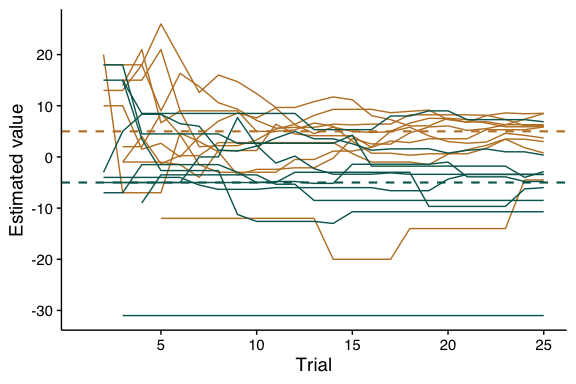
\includegraphics{hot_stove_sims_files/figure-latex/unnamed-chunk-16-1.pdf}

\begin{Shaded}
\begin{Highlighting}[]
\NormalTok{numrep\_choices\_df }\OtherTok{\textless{}{-}}\NormalTok{ simsdf }\SpecialCharTok{\%\textgreater{}\%}
  \FunctionTok{group\_by}\NormalTok{(tau, sim) }\SpecialCharTok{\%\textgreater{}\%}
  \FunctionTok{filter}\NormalTok{(choice }\SpecialCharTok{==} \DecValTok{2}\NormalTok{) }\SpecialCharTok{\%\textgreater{}\%}
  \FunctionTok{mutate}\NormalTok{(}
    \AttributeTok{arm2\_chosen\_again =} \FunctionTok{n}\NormalTok{() }\SpecialCharTok{{-}} \DecValTok{1}\NormalTok{,}
    \AttributeTok{first\_rew\_arm2 =} \FunctionTok{first}\NormalTok{(rew\_arm2),}
    \AttributeTok{first\_rew\_arm2\_quant =} \FunctionTok{ntile}\NormalTok{(first\_rew\_arm2, }\DecValTok{20}\NormalTok{)) }\SpecialCharTok{\%\textgreater{}\%}
  \FunctionTok{group\_by}\NormalTok{(tau,first\_rew\_arm2\_quant) }\SpecialCharTok{\%\textgreater{}\%}
  \FunctionTok{summarise}\NormalTok{(}\AttributeTok{arm2\_chosen\_again =} \FunctionTok{mean}\NormalTok{(arm2\_chosen\_again)) }\SpecialCharTok{\%\textgreater{}\%}
  \FunctionTok{arrange}\NormalTok{(tau,first\_rew\_arm2\_quant)}
\end{Highlighting}
\end{Shaded}

\begin{verbatim}
## `summarise()` has grouped output by 'tau'. You can override using the `.groups`
## argument.
\end{verbatim}

\begin{Shaded}
\begin{Highlighting}[]
\FunctionTok{ggplot}\NormalTok{(numrep\_choices\_df, }\FunctionTok{aes}\NormalTok{(}\AttributeTok{x=}\NormalTok{first\_rew\_arm2\_quant,}\AttributeTok{y=}\NormalTok{arm2\_chosen\_again)) }\SpecialCharTok{+}
  \FunctionTok{geom\_line}\NormalTok{(}\FunctionTok{aes}\NormalTok{(}\AttributeTok{color=}\FunctionTok{as.factor}\NormalTok{(tau)), }\AttributeTok{size=}\DecValTok{1}\NormalTok{) }\SpecialCharTok{+}
\NormalTok{  paltau\_color }\SpecialCharTok{+} 
\NormalTok{  paltau\_fill }\SpecialCharTok{+}
  \FunctionTok{xlab}\NormalTok{(}\StringTok{"Reward after arm 2 is first chosen, quantile"}\NormalTok{) }\SpecialCharTok{+}
  \FunctionTok{ylab}\NormalTok{(}\StringTok{"Times arm 2 is chosen again"}\NormalTok{) }\SpecialCharTok{+}
  \FunctionTok{theme}\NormalTok{(}
    \AttributeTok{legend.position =} \FunctionTok{c}\NormalTok{(}\FloatTok{0.75}\NormalTok{, }\FloatTok{0.1}\NormalTok{),}
    \AttributeTok{legend.direction =} \StringTok{"horizontal"}\NormalTok{)}
\end{Highlighting}
\end{Shaded}

\begin{verbatim}
## Warning in grid.Call(C_textBounds, as.graphicsAnnot(x$label), x$x, x$y, : font
## metrics unknown for Unicode character U+03c4

## Warning in grid.Call(C_textBounds, as.graphicsAnnot(x$label), x$x, x$y, : font
## metrics unknown for Unicode character U+03c4

## Warning in grid.Call(C_textBounds, as.graphicsAnnot(x$label), x$x, x$y, : font
## metrics unknown for Unicode character U+03c4

## Warning in grid.Call(C_textBounds, as.graphicsAnnot(x$label), x$x, x$y, : font
## metrics unknown for Unicode character U+03c4

## Warning in grid.Call(C_textBounds, as.graphicsAnnot(x$label), x$x, x$y, : font
## metrics unknown for Unicode character U+03c4

## Warning in grid.Call(C_textBounds, as.graphicsAnnot(x$label), x$x, x$y, : font
## metrics unknown for Unicode character U+03c4

## Warning in grid.Call(C_textBounds, as.graphicsAnnot(x$label), x$x, x$y, : font
## metrics unknown for Unicode character U+03c4

## Warning in grid.Call(C_textBounds, as.graphicsAnnot(x$label), x$x, x$y, : font
## metrics unknown for Unicode character U+03c4

## Warning in grid.Call(C_textBounds, as.graphicsAnnot(x$label), x$x, x$y, : font
## metrics unknown for Unicode character U+03c4

## Warning in grid.Call(C_textBounds, as.graphicsAnnot(x$label), x$x, x$y, : font
## metrics unknown for Unicode character U+03c4

## Warning in grid.Call(C_textBounds, as.graphicsAnnot(x$label), x$x, x$y, : font
## metrics unknown for Unicode character U+03c4

## Warning in grid.Call(C_textBounds, as.graphicsAnnot(x$label), x$x, x$y, : font
## metrics unknown for Unicode character U+03c4

## Warning in grid.Call(C_textBounds, as.graphicsAnnot(x$label), x$x, x$y, : font
## metrics unknown for Unicode character U+03c4

## Warning in grid.Call(C_textBounds, as.graphicsAnnot(x$label), x$x, x$y, : font
## metrics unknown for Unicode character U+03c4

## Warning in grid.Call(C_textBounds, as.graphicsAnnot(x$label), x$x, x$y, : font
## metrics unknown for Unicode character U+03c4

## Warning in grid.Call(C_textBounds, as.graphicsAnnot(x$label), x$x, x$y, : font
## metrics unknown for Unicode character U+03c4

## Warning in grid.Call(C_textBounds, as.graphicsAnnot(x$label), x$x, x$y, : font
## metrics unknown for Unicode character U+03c4

## Warning in grid.Call(C_textBounds, as.graphicsAnnot(x$label), x$x, x$y, : font
## metrics unknown for Unicode character U+03c4

## Warning in grid.Call(C_textBounds, as.graphicsAnnot(x$label), x$x, x$y, : font
## metrics unknown for Unicode character U+03c4

## Warning in grid.Call(C_textBounds, as.graphicsAnnot(x$label), x$x, x$y, : font
## metrics unknown for Unicode character U+03c4

## Warning in grid.Call(C_textBounds, as.graphicsAnnot(x$label), x$x, x$y, : font
## metrics unknown for Unicode character U+03c4

## Warning in grid.Call(C_textBounds, as.graphicsAnnot(x$label), x$x, x$y, : font
## metrics unknown for Unicode character U+03c4

## Warning in grid.Call(C_textBounds, as.graphicsAnnot(x$label), x$x, x$y, : font
## metrics unknown for Unicode character U+03c4

## Warning in grid.Call(C_textBounds, as.graphicsAnnot(x$label), x$x, x$y, : font
## metrics unknown for Unicode character U+03c4

## Warning in grid.Call(C_textBounds, as.graphicsAnnot(x$label), x$x, x$y, : font
## metrics unknown for Unicode character U+03c4

## Warning in grid.Call(C_textBounds, as.graphicsAnnot(x$label), x$x, x$y, : font
## metrics unknown for Unicode character U+03c4

## Warning in grid.Call(C_textBounds, as.graphicsAnnot(x$label), x$x, x$y, : font
## metrics unknown for Unicode character U+03c4

## Warning in grid.Call(C_textBounds, as.graphicsAnnot(x$label), x$x, x$y, : font
## metrics unknown for Unicode character U+03c4

## Warning in grid.Call(C_textBounds, as.graphicsAnnot(x$label), x$x, x$y, : font
## metrics unknown for Unicode character U+03c4

## Warning in grid.Call(C_textBounds, as.graphicsAnnot(x$label), x$x, x$y, : font
## metrics unknown for Unicode character U+03c4

## Warning in grid.Call(C_textBounds, as.graphicsAnnot(x$label), x$x, x$y, : font
## metrics unknown for Unicode character U+03c4

## Warning in grid.Call(C_textBounds, as.graphicsAnnot(x$label), x$x, x$y, : font
## metrics unknown for Unicode character U+03c4

## Warning in grid.Call(C_textBounds, as.graphicsAnnot(x$label), x$x, x$y, : font
## metrics unknown for Unicode character U+03c4

## Warning in grid.Call(C_textBounds, as.graphicsAnnot(x$label), x$x, x$y, : font
## metrics unknown for Unicode character U+03c4

## Warning in grid.Call(C_textBounds, as.graphicsAnnot(x$label), x$x, x$y, : font
## metrics unknown for Unicode character U+03c4

## Warning in grid.Call(C_textBounds, as.graphicsAnnot(x$label), x$x, x$y, : font
## metrics unknown for Unicode character U+03c4

## Warning in grid.Call(C_textBounds, as.graphicsAnnot(x$label), x$x, x$y, : font
## metrics unknown for Unicode character U+03c4

## Warning in grid.Call(C_textBounds, as.graphicsAnnot(x$label), x$x, x$y, : font
## metrics unknown for Unicode character U+03c4

## Warning in grid.Call(C_textBounds, as.graphicsAnnot(x$label), x$x, x$y, : font
## metrics unknown for Unicode character U+03c4

## Warning in grid.Call(C_textBounds, as.graphicsAnnot(x$label), x$x, x$y, : font
## metrics unknown for Unicode character U+03c4

## Warning in grid.Call(C_textBounds, as.graphicsAnnot(x$label), x$x, x$y, : font
## metrics unknown for Unicode character U+03c4

## Warning in grid.Call(C_textBounds, as.graphicsAnnot(x$label), x$x, x$y, : font
## metrics unknown for Unicode character U+03c4

## Warning in grid.Call(C_textBounds, as.graphicsAnnot(x$label), x$x, x$y, : font
## metrics unknown for Unicode character U+03c4

## Warning in grid.Call(C_textBounds, as.graphicsAnnot(x$label), x$x, x$y, : font
## metrics unknown for Unicode character U+03c4

## Warning in grid.Call(C_textBounds, as.graphicsAnnot(x$label), x$x, x$y, : font
## metrics unknown for Unicode character U+03c4

## Warning in grid.Call(C_textBounds, as.graphicsAnnot(x$label), x$x, x$y, : font
## metrics unknown for Unicode character U+03c4

## Warning in grid.Call(C_textBounds, as.graphicsAnnot(x$label), x$x, x$y, : font
## metrics unknown for Unicode character U+03c4

## Warning in grid.Call(C_textBounds, as.graphicsAnnot(x$label), x$x, x$y, : font
## metrics unknown for Unicode character U+03c4
\end{verbatim}

\begin{verbatim}
## Warning in grid.Call.graphics(C_text, as.graphicsAnnot(x$label), x$x, x$y, :
## font metrics unknown for Unicode character U+03c4

## Warning in grid.Call.graphics(C_text, as.graphicsAnnot(x$label), x$x, x$y, :
## font metrics unknown for Unicode character U+03c4
\end{verbatim}

\begin{verbatim}
## Warning in grid.Call.graphics(C_text, as.graphicsAnnot(x$label), x$x, x$y, :
## conversion failure on 'τ' in 'mbcsToSbcs': dot substituted for <cf>
\end{verbatim}

\begin{verbatim}
## Warning in grid.Call.graphics(C_text, as.graphicsAnnot(x$label), x$x, x$y, :
## conversion failure on 'τ' in 'mbcsToSbcs': dot substituted for <84>
\end{verbatim}

\includegraphics{hot_stove_sims_files/figure-latex/unnamed-chunk-17-1.pdf}

\end{document}
